\chapter{The concept of black hole 2: Non-expanding horizons and Killing horizons}
\label{s:neh}

\minitoc

\section{Introduction}

Having discussed in depth the geometry of null hypersurfaces in Chap.~\ref{s:def}
we move forward to distinguish a null hypersurface representing a black hole event horizon from, let us say, that representing a mere future light cone. We do it here for black holes
\emph{in equilibrium}. Indeed, for such objects, it is quite natural
to assume a vanishing expansion. This leads us to the concept of \emph{non-expanding
horizon} (Sec.~\ref{s:neh:neh}). A special kind of these objects is that
of \emph{Killing horizons} (Sec.~\ref{s:neh:Killing_hor}). Actually, we shall
see in Chap.~\ref{s:sta} that the event horizon of a black hole in equilibrium
must be a Killing horizon.


%%%%%%%%%%%%%%%%%%%%%%%%%%%%%%%%%%%%%%%%%%%%%%%%%%%%%%%%%%%%%%%%%%%%%%%%%%%%%%%%%%%%%%%%

\section{Non-expanding horizons} \label{s:neh:neh}

\subsection{Motivation and definition}

In Chap.~\ref{s:def}, the null hypersurfaces have been introduced as boundaries
of black holes, from the ``no-escape'' aspect of the naive definition given in
Sec.~\ref{s:def:first_defin}. To enforce the ``localized'' facet of the definition,
we could demand that the cross-sections are closed (compact without boundary\footnote{Cf. the discussion in Sec.~\ref{s:def:spacelike_sections}.})
and have a constant area, i.e. a vanishing expansion. Hence the definition:
\begin{greybox}
A \defin{non-expanding horizon}\index{non-expanding!horizon}\index{horizon!non-expanding --} is a null hypersurface $\Hor$ having the
topology (\ref{e:def:H_topology}):
\be
    \Hor \simeq \R \times \Sp,
\ee
where $\Sp$ is a closed manifold\index{closed!manifold} of dimension $n-2$,
and such that the expansion of $\Hor$ along any null normal $\wl$ vanishes
identically:
\be
    \theta_{(\wl)} = 0 .
\ee
\end{greybox}
\begin{remark}
Note that, given the scaling law (\ref{e:def:rescale_lambda}),
if $\theta_{(\wl)} = 0$ for some normal $\wl$, then  $\theta_{(\wl')} = 0$
for any other normal $\wl'$. Hence the definition of a non-expanding horizon
does not depend on the choice of the null normal.
\end{remark}
As we shall discuss in detail in Chap.~\ref{s:sta}, this definition captures only
the event horizon of black holes in equilibrium. For a black hole out of equilibrium,
one has generically $\theta_{(\wl)} > 0$.

\begin{example}[Schwarzschild horizon]
In view of Eq.~(\ref{e:def:theta_Schw_hor}), we may assert that the
Schwarz\-schild horizon considered in Examples~\ref{x:def:Schw_hor}, \ref{x:def:Schw_hor2},
\ref{x:def:Schw_hor3}, \ref{x:def:Schw_hor4}, \ref{x:def:Schw_hor5}, \ref{x:def:Schw_hor6},
\ref{x:def:Schw_hor7}, \ref{x:def:Schw_hor8} and \ref{x:def:Schw_hor9}
of Chap.~\ref{s:def}
is a non-expanding horizon.
\end{example}

\begin{example}[null hyperplane and light cone as counter-examples]
The null hyperplane and light cone in Minkowski spacetime considered
in the examples of Chap.~\ref{s:def} are excluded by the above definition,
having non-compact cross-sections (null hyperplane) or nonzero expansion
(light cone).
\end{example}

\begin{hist}\label{h:neh:NEH}
The concept of non-expanding horizon has been introduced by
Petr~H\'a\'\j i\v{c}ek\index{Hajicek, P.@Ha\'\j i\v{c}ek, P.}
in 1973 under the name of \emph{totally geodesic null hypersurface} \cite{Hajic73a}
or \emph{perfect horizon} \cite{Hajic73b,Hajic74}.
The terminology \emph{non-expanding horizon} is due to
Abhay Ashtekar\index{Ashtekar, A.}, Stephen Fairhurst\index{Fairhurst, S.}
and Badri Krishnan\index{Krishnan, B.} in 2000 \cite{AshteFK00} (see also \cite{AshteBL02}).
\end{hist}

\subsection{Invariance of the area} \label{s:neh:invar_area}

Given a cross-section $\Sp$ of $\Hor$, the area\index{area!of a cross-section} of $\Sp$, with respect to the spacetime metric $\w{g}$, is [cf. Eqs.~(\ref{e:def:A_wepsS_dx}) and (\ref{e:def:A_sqrt_q})]
\be \label{e:neh:total_area}
    A = \int_{\Sp} \wepsS(\D\w{x}_{(2)},\ldots,\D\w{x}_{(n-1)})
        = \int_{\Sp} \sqrt{q} \, \D x^2 \cdots \D x^{n-1} ,
\ee
where $x^a = (x^2, \ldots, x^{n-1})$ is a coordinate system on $\Sp$ and $q$ is
the determinant with respect to these coordinates of the Riemannian metric $\w{q}$
induced by $\w{g}$ on $\Sp$.

A direct consequence of the definition of a non-expanding horizon is that
$A$ does not depend on the choice of the cross-section $\Sp$.
\begin{proof}
Let $\Sp'$ be a second cross-section of $\Hor$ and let $\wl$ be a field of null normals
of $\Hor$. Along the null geodesic generators of $\Hor$, we can always choose a parameter $\lambda$ associated with $\wl$ (i.e. such that $\wl = \D/\D\lambda$ along a given null geodesic generator)
such that $\lambda=0$ on $\Sp$. By the very definition of a cross-section,
any null geodesic generator $\Li$ of $\Hor$ intersects $\Sp'$ at a single point. Let
$\lambda_0$ be the value of $\lambda$ at this point. We may then introduce
a new parameter along $\Li$ as follows:
\[
      \lambda' = \frac{\lambda}{\lambda_0} .
\]
If we repeat this for all null geodesic generators of $\Hor$, we obtain a parametrization
of all the null geodesic generators that satisfies $\lambda'=0$ on $\Sp$ and $\lambda'=1$
on $\Sp'$. Let $\wl'=\D/\D\lambda'$ be the (null) tangent vector associated
with $\lambda'$. We may then say that the cross-section $\Sp'$ is deduced
from $\Sp$ by the Lie dragging of $\Sp$ along $\wl'$ by a parameter $\delta\lambda'=1$.
More precisely, we may consider that $\Sp'$ is deduced from $\Sp$ by a
continuous deformation, represented by a 1-parameter family $(\Sp_{\lambda'})$
of cross-sections such that $\Sp_0 = \Sp$ and $\Sp_1 = \Sp'$. Associated
with this family is a real-valued function $\lambda' \mapsto A(\lambda')$
given the area of each element $\Sp_{\lambda'}$. By the very definition
of the expansion along $\wl'$ [Eq.~(\ref{e:def:def_expansion})], we have then
\[
    \frac{\D A}{\D\lambda'} = \int_{\Sp_{\lambda'}} \theta_{(\wl')} \, \delta A .
\]
If $\Hor$ is a non-expanding horizon, then $\theta_{(\wl')}=0$ and it follows
that $A(\lambda')$ is a constant function. Hence the area of $\Sp'$ is equal
to that of $\Sp$.
\end{proof}
\begin{greybox}
Given that the quantity $A$ defined by (\ref{e:neh:total_area})
takes a unique value whatever the cross-section $\Sp$,
we call it the \defin{area of the non-expanding horizon}\index{area!of a non-expanding horizon}
$\Hor$.
\end{greybox}

\begin{example}[Schwarzschild horizon] \label{x:neh:Schwarz_hor_area}
The area of the Schwarzschild horizon is readily computed from
the metric (\ref{e:def:q_S_Schw_hor}):
$q_{ab} \D x^a \D x^b = 4m^2 \left( \D\th^2 + \sin^2\th \D^2\ph \right)$;
we get
\[
     A = 16\pi m^2 .
\]
\end{example}

\subsection{Trapped surfaces}

If there exists some natural concept of \emph{outer}/\emph{inner} for $\Hor$, for
instance the outer region being the one that contains an asymptotically flat end,
and if the transverse null normals $\w{k}$ to cross-sections point to the inner region, then
the property $\theta_{(\wl)}=0$ means that any cross-section $\Sp$ of the
non-expanding horizon $\Hor$ is a
\defin{marginally outer trapped surface}\index{marginally!outer trapped surface}\index{trapped!surface!marginally outer --}
(often abridged as \defin{MOTS}\index{MOTS}). This definition is due to
Hawking \cite{Hawki73}, an
\defin{outer trapped surface}\index{outer!trapped surface}\index{trapped!surface!outer --}
would be one for which $\theta_{(\wl)}\leq 0$.

\begin{figure}
\centerline{\includegraphics[width=0.36\textwidth]{neh_trapped_surf.pdf}\ \qquad \
\includegraphics[width=0.52\textwidth]{neh_untrapped_surf.pdf}
}
\caption[]{\label{f:neh:trapped_surf} \footnotesize
Trapped surface (left): $\delta A^{(\wl)}_\varepsilon  < \delta A$
and untrapped surface (right): $\delta A^{(\wl)}_\varepsilon  > \delta A$,
both surfaces having $\delta A^{(\w{k})}_\varepsilon  < \delta A$.
}
\end{figure}


The MOTS definition is related to, but distinct from, the definition of a
marginally trapped surface by Penrose \cite{Penro65}: a $(n-2)$-dimensional
submanifold $\Sp$ of $\M$ is a \defin{trapped surface}\index{trapped!surface}
 iff (i) $\Sp$ is
closed (i.e. compact without boundary), (ii) $\Sp$ is spacelike and (iii)
the two systems of null geodesics emerging orthogonally from $\Sp$ converge
locally at $\Sp$, i.e. they have negative expansions:
\be
    \theta_{(\wl)} < 0 \quad\mbox{and}\quad \theta_{(\w{k})} < 0 ,
\ee
where the expansion along $\w{k}$ is defined in the same way as that along
$\wl$ [cf. Eq.~(\ref{e:def:theta_l_all})]:
\be \label{e:neh:expansion_k}
    \theta_{(\w{k})} := \lim_{\varepsilon\rightarrow 0} \frac{1}{\varepsilon}
    \frac{\delta A^{(\w{k})}_\varepsilon - \delta A}{\delta A}
        = \frac{1}{2} \Lie{\w{k}} \ln q
        = \frac{1}{2} \, q^{\mu\nu} \Liec{k} q_{\mu\nu}
        = q^{\mu\nu} \nabla_\mu k_\nu ,
\ee
$\delta A^{(\w{k})}_\varepsilon$ being the area of the surface element
that is deduced from the surface element of area $\delta A$ on $\Sp$ by the
Lie dragging along $\w{k}$ by a parameter $\varepsilon$ (cf. Fig.~\ref{f:neh:trapped_surf} left).
The limit case $\theta_{(\wl)} = 0$ and $\theta_{(\w{k})}<0$ correspond
to the so-called \defin{marginally trapped surface}\index{marginally!trapped surface}.

In flat spacetime (Minkowski), given any closed spacelike surface,
one has $\theta_{(\wl)} > 0$ and $\theta_{(\w{k})} < 0$ (cf. Fig.~\ref{f:neh:trapped_surf} right), so there
is no trapped surface.

\begin{remark}
The hypothesis of \emph{closed} surface is crucial in the definition of a
trapped surface. For instance, there are non-closed spacelike surfaces in
Minkowski spacetime having $\theta_{(\wl)} < 0$ and $\theta_{(\w{k})} < 0$.
A well known such example is the intersection of two past null cones (see e.g.
Fig.~5.13 of \cite{FroloN98}).
\end{remark}

Cross-sections of a non-expanding horizon are usually marginally trapped surfaces
(cf. the example below).
However, there exist some pathological situations for
which $\theta_{(\w{k})} > 0$ at some points of $\Sp$ \cite{GerocH82}.

\begin{example}
Let us consider a cross-section $\Sp$ of the Schwarzschild horizon as
defined in Example~\ref{x:def:Schw_hor4} of Chap.~\ref{s:def}.
Computing $q^{\mu\nu} \nabla_\mu k_\nu$ from the components $k_\nu$
given by (\ref{e:def:l_k_forms_Schw_hor}) we get (cf. Sec.~\ref{s:sam:Schwarz_hor} for
the computation)
\[
    \theta_{(\w{k})} = - \frac{r+2m}{r^2} .
\]
In particular, on $\Sp$ ($r=2m$),
\[
    \theta_{(\w{k})}  = - \frac{1}{m} .
\]
Hence $\theta_{(\w{k})} < 0$. Since we had already $\theta_{(\wl)}=0$
[cf. Eq.~(\ref{e:def:theta_Schw_hor})], we conclude that $\Sp$ is a
marginally trapped surface. This could also have been inferred from
Fig.~\ref{f:def:Schw_hor_lk}, since according to the metric
(\ref{e:def:q_Schw_hor}), the area of the cross-sections of $\Hor$
is nothing but $4\pi r^2$ and $\w{k}$ points to decreasing values of $r$, while, on $\Hor$,
$\wl$ points to a fixed value of $r$.
\end{example}

\subsection{Vanishing of the deformation rate tensor} \label{s:neh:NEH_Theta_zero}

If $\Hor$ is a non-expanding horizon, we may set $\theta_{(\wl)}=0$
in the null Raychaudhuri equation (\ref{e:def:null_Raychaud}); it reduces then
to
\be \label{e:neh:null_Raychaud_theta_zero}
    \sigma_{ab} \sigma^{ab} + 8\pi \w{T}(\wl, \wl) = 0 .
\ee
Now, the first term is always non-negative:
\be \label{e:neh:sigma_square}
    \sigma_{ab} \sigma^{ab} \geq 0 .
\ee
\begin{proof}
Since $\w{\sigma}$ is symmetric, it can be diagonalized
in an orthonormal basis of $\w{q}$: $\sigma_{ab} = \mathrm{diag}(s_1,\ldots, s_{n-2})$.
Moreover, $\w{q}$ being a Riemannian metric, we have, in the same basis, $q^{ab} = \mathrm{diag}(1,\ldots,1)$. Since $\sigma^{ab} = q^{am} q^{bn} \sigma_{mn}$, we conclude that
\be \label{e:neh:sigma_square_si}
  \sigma_{ab} \sigma^{ab} = s_1^2 + \cdots + s_{n-2}^2 \geq 0 .
\ee
\end{proof}

Regarding the second term in (\ref{e:neh:null_Raychaud_theta_zero}), it
is quite natural to assume that matter and non-gravitational fields,
represented by the total energy-momentum tensor $\w{T}$, obey the
\defin{null energy condition}\index{null!energy condition}\index{energy!condition!null --},
namely that
\be \label{e:neh:null_energy_cond}
    \w{T}(\wl, \wl) \geq 0 \quad \mbox{for any null vector $\wl$}.
\ee
This condition is pretty weak and is satisfied by
\begin{itemize}
\item vacuum: $\w{T}=0$;
\item any ``reasonable'' matter model, such as a perfect fluid with a
proper energy density $\varepsilon$ and pressure $p$ satisfying\footnote{Indeed, from the form $\w{T} = (\varepsilon+p)\uu{u}\otimes\uu{u} + p \w{g}$
of the energy-momentum tensor of a perfect fluid, one has
$\w{T}(\wl,\wl) = (\varepsilon+p)(\w{u}\cdot\wl)^2$ with $(\w{u}\cdot\wl)^2\geq 0$.}
$\varepsilon+p\geq 0$;
\item any electromagnetic field;
\item any real or complex scalar field;
\item ``dark energy''\index{dark energy} modelled by $\w{T} = -\frac{\Lambda}{8\pi}\, \w{g}$.
\end{itemize}
Note also that the null energy condition is implied by the
so-called \defin{weak energy condition}\index{weak!energy condition}\index{energy!condition!weak --},
which states that
\be
    \w{T}(\w{u}, \w{u}) \geq 0 \quad \mbox{for any timelike vector $\w{u}$}.
\ee
The null energy condition follows from the
weak energy condition by continuity.
Selecting for $\w{u}$ the 4-velocity of an observer, we see that
the weak energy condition has a simple physical interpretation: the energy
density as measured by any observer is non-negative.

Given (\ref{e:neh:sigma_square}) and (\ref{e:neh:null_energy_cond}),
Eq.~(\ref{e:neh:null_Raychaud_theta_zero})  implies both
\be
    \sigma_{ab} \sigma^{ab}  = 0
\ee
and
\be \label{e:neh:T_l_l_zero}
    \w{T}(\wl, \wl) = 0 .
\ee
The identity $\sigma_{ab} \sigma^{ab} = 0$ is possible only if each of
the $s_i$'s in (\ref{e:neh:sigma_square_si}) is zero. Hence we have necessarily
\be
    \w{\sigma} = 0 .
\ee
Since we had already $\theta_{(\wl)}=0$ (non-expanding horizon), this implies that the full deformation rate tensor
vanishes identically [cf. Eq.~(\ref{e:def:def_shear})]:
\be
    \w{\Theta} = 0 .
\ee
In view of (\ref{e:def:Theta}), this is equivalent to
\be \label{e:neh:Lie_el_q_zero}
     \vw{q}^* \Lie{\el} \w{q} = 0 .
\ee
We conclude that, provided that the null energy condition holds,
the whole metric (and not only the area element
$\wepsS$, as a mere $\theta_{(\wl)}=0$ would suggest) of any cross-section
of a non-expanding horizon is invariant along the null geodesic generators.

\begin{example}[Schwarzschild horizon]
We had already noticed that, for the Schwarzschild horizon, $\w{\Theta}=0$
[Eq.~(\ref{e:def:Theta_zero_Schw_hor}) in Example~\ref{x:def:Schw_hor8}
of Chap.~\ref{s:def}].
\end{example}

\subsection{Induced affine connection} \label{e:neh:induced_connection}

Since $\Hor$ is a null hypersurface, the ``metric'' $\left. \w{g}\right|_{\Hor}$
induced on it by the spacetime metric $\w{g}$ is degenerate. As a consequence, there
is a priori no unique connection on $\Hor$ associated with it. However, when
$\Hor$ is a non-expanding horizon and the null energy condition holds on $\Hor$,
so that $\w{\Theta}=0$, the spacetime connection $\wnab$ induces a unique
connection ${}^\Hor\!\wnab$ on $\Hor$ as follows.
Let $\w{u}$ and $\w{v}$ be two vector fields on $\Hor$. We have, using
(\ref{e:def:nab_l_Theta}) to express $\nabla_\nu \el_\mu$ in terms of $\Theta_{\nu\mu}$:
\bea
    \el_\mu u^\nu \nabla_\nu v^\mu &= &
        u^\nu \nabla_\nu ( \underbrace{\el_\mu v^\mu}_{0} )
        - v^\mu u^\nu \nabla_\nu \el_\mu \nonumber \\
        & = & - \underbrace{\Theta_{\nu\mu}}_{0} v^\mu u^\nu  - \omega_\nu u^\nu
            \underbrace{\el_\mu v^\mu}_{0}
            + v^\mu \underbrace{u^\nu \el_\nu}_{0} k^\sigma\nabla_\sigma \el_\mu
             = 0    \nonumber .
\eea
Hence $\wl$ is orthogonal to the vector field $\wnab_{\w{u}} \w{v}$. It follows
immediately that $\wnab_{\w{u}} \w{v}$ is tangent to $\Hor$.
We conclude that the operator
\be \label{e:neh:def_induced_connection}
    \begin{array}{cccc}
    {}^\Hor\!\wnab \ : & \mathfrak{X}(\Hor)\times\mathfrak{X}(\Hor) & \longrightarrow & \mathfrak{X}(\Hor) \\
    & (\w{u},\w{v}) & \longmapsto & \wnab_{\w{u}} \,\w{v} ,
    \end{array}
\ee
where $\mathfrak{X}(\Hor)$ is the space of vector fields on $\Hor$, is
well-defined (i.e. ${}^\Hor\!\wnab_{\w{u}}\w{v}$  does belong to
$\mathfrak{X}(\Hor)$).
Moreover, this operator fulfills all the properties of an affine connection
(cf. Sec.~\ref{s:bas:affine_connect}), since $\wnab$ does.
We naturally call ${}^\Hor\!\wnab$ the \defin{affine connection induced on $\Hor$
by}\index{induced! affine connection}\index{affine connection!induced --}\index{connection!induced --} $\wnab$.

A geometrical consequence of the identity
${}^\Hor\!\wnab_{\w{u}}\w{v} = \wnab_{\w{u}}\w{v}$ is
that $(\Hor, {}^\Hor\!\wnab)$ is a \defin{totally geodesic submanifold}\index{totally geodesic} of $(\M,\w{g})$:
i.e. any geodesic of $(\Hor, {}^\Hor\!\wnab)$ is also a geodesic of $(\M,\w{g})$
(cf. the historical note on page~\pageref{h:neh:NEH}).

The covariant derivative of the null normal $\wl$ with respect to the affine
connection ${}^\Hor\!\wnab$ takes a rather simple form:
\be \label{e:neh:nabH_ell}
   \encadre{ {}^\Hor\!\wnab \wl = \wl \otimes {}^\Hor\!\w{\omega} },
\ee
where ${}^\Hor\!\w{\omega}$ is the tensor field on $\Hor$
defined as the restriction of the 1-form $\w{\omega}$
introduced in Sec.~\ref{s:def:deformation_shear}
to vectors tangent to $\Hor$ [cf. Eq.~(\ref{e:def:omega_restrict_H})].
In other words, ${}^\Hor\!\w{\omega}$ is the pullback $\iota^*\w{\omega}$ of
$\w{\omega}$ by the inclusion map $\iota: \Hor \to \M$ (cf. Sec.~\ref{s:bas:lie_der_tensor}
in Appendix~\ref{s:bas}).
\begin{proof}
By definition of the covariant derivative with respect to an
affine connection [cf. Eq.~(\ref{e:bas:def_cov_deriv}) in Appendix~\ref{s:bas}],
${}^\Hor\!\wnab \wl$ is a tensor field of type $(1,1)$ on $\Hor$,
the action of which on any pair
$(\w{a}, \w{u})$ formed by a 1-form $\w{a}$ and a vector field $\w{u}$
on $\Hor$ is
\[
    {}^\Hor\!\wnab \wl (\w{a}, \w{u}) = \langle \w{a}, {}^\Hor\!\wnab_{\w{u}} \wl \rangle .
\]
In view of (\ref{e:neh:def_induced_connection}) and using Eq.~(\ref{e:def:nab_l_Theta})
to express $\wnab\wl$, we get
\begin{align}
    {}^\Hor\!\wnab \wl (\w{a}, \w{u}) & = \langle \w{a}, \wnab_{\w{u}} \wl \rangle
       = a_\mu u^\nu \nabla_\nu \ell^\mu \nonumber \\
        & = a_\mu u^\nu \Big( \underbrace{\Theta^\mu_{\ \, \nu}}_{0} + \omega_\nu \ell^\mu
            - \ell_\nu k^\rho \nabla_\rho \ell^\mu \Big)
         = a_\mu \ell^\mu \, \omega_\nu u^\nu - \underbrace{\ell_\nu u^\nu}_{0}
            a_\mu k^\rho \nabla_\rho \ell^\mu \nonumber \\
         & = \langle \w{a}, \wl \rangle \, \langle \w{\omega}, \w{u} \rangle . \nonumber
\end{align}
Given the definition of a tensor product and the fact that $\w{u}$ is tangent to $\Hor$,
this proves (\ref{e:neh:nabH_ell}).
\end{proof}
A priori the 1-form ${}^\Hor\!\w{\omega}$ depends upon the choice of the cross-section $\Sp$
of $\Hor$, via the vector $\w{k}$ involved in Eq.~(\ref{e:def:omega_restrict_H}):
$\langle {}^\Hor\!\w{\omega}, \w{v} \rangle = - \w{k} \cdot\wnab_{\w{v}} \w{\ell}$
for any $\w{v}\in T_p\Hor$. Formula~(\ref{e:neh:nabH_ell}) shows that for a non-expanding
horizon, this is not the case: ${}^\Hor\!\w{\omega}$ is  a quantity intrinsic to $\Hor$ and to the value of $\wl$ on $\Hor$.
Moreover, under a change of null normal, $\wl \mapsto \wl' = \alpha \wl$,
it remains constant up to the addition of an exact 1-form:
${}^\Hor\!\w{\omega}' = {}^\Hor\!\w{\omega} + \dd\ln\alpha$.
The 1-form ${}^\Hor\!\w{\omega}$
is usually called the \defin{rotation 1-form} or \defin{connection 1-form}
of $(\Hor, \wl)$ \cite{AshteBL02,GourgJ06}.

\subsection{Going further}

See Refs.~\cite{AshteK04,GourgJ06,Jaram13} for more
about non-expanding horizons, in particular for a subclass of them
called \emph{isolated horizons}\index{isolated!horizon}\index{horizon!isolated}.


%%%%%%%%%%%%%%%%%%%%%%%%%%%%%%%%%%%%%%%%%%%%%%%%%%%%%%%%%%%%%%%%%%%%%%%%%%%%%%%

\section{Killing horizons} \label{s:neh:Killing_hor}

A special kind of non-expanding horizons, which is of primordial
importance for the theory of
stationary black holes, is that of Killing horizons with closed-manifold cross-sections.
Defining a Killing horizon requires the concepts of \emph{1-dimensional group of
isometries} and \emph{Killing vector}, which we discuss first.

\begin{figure}
\centerline{\includegraphics[width=0.8\textwidth]{def_group_action.pdf}}
\caption[]{\label{f:neh:group_action} \footnotesize
Group action of $G$ on $\M$.}
\end{figure}


\subsection{Spacetime symmetries} \label{s:neh:symmetries}

Symmetries of spacetime are described in a coordinate-independent way by means of
a (symmetry) group acting on the spacetime manifold $\M$.
Through this action, each transformation belonging to the group displaces points within $\M$ and one demands that the metric $\w{g}$ is invariant under such displacement.
More precisely, given
a group $G$, a \defin{group action}\index{group!action} of $G$ on $\M$ is a map\footnote{Do no confuse the generic element $g$ of group $G$ with the metric tensor $\w{g}$.}
\be
    \begin{array}{rccl}
    \Phi: & G\times \M & \longrightarrow & \M \\
        & (g,p) & \longmapsto & \Phi(g,p) =: \Phi_g(p)
    \end{array}
\ee
such that (cf. Fig.~\ref{f:neh:group_action})
\begin{itemize}
\item $\forall p\in \M,\  \Phi_e(p) = p$, where $e$ is the identity element of $G$;
\item $\forall (g,h) \in G^2,\  \forall p\in\M,\  \Phi_g(\Phi_h(p)) = \Phi_{gh}(p)$, where $gh$ stands for the product of $g$ by $h$ according to $G$'s group law.
\end{itemize}
The \defin{orbit}\index{orbit!under a group action} of a point $p\in\M$ is the set $\{g(p),\ g\in G\}\subset\M$, i.e. the set of points which are connected to $p$ by some group transformation. One says that $p$ is a
\defin{fixed point}\index{fixed!point} of the group action if its orbit is
reduced to $\{p\}$.

An important class of group actions are those for which $G$ is a 1-dimensional
\emph{Lie group}, i.e. a ``continuous'' group (actually a ``differentiable'' group).
Then around $e$, the elements of $G$ can be labelled by a parameter $t\in \R$, such that $g_{t=0} = e$. It is then
common to use the shorthand notation
\be
        \Phi_t := \Phi_{g_t} .
\ee
Because $G$ is a 1-dimensional Lie group, the orbit of a given point $p\in\M$ under the group action is then either $\{p\}$ (when $p$ is fixed point of the
group action) or a curve of $\M$. In the latter case,
$t$ is a natural parameter along the curve (cf. Fig.~\ref{f:neh:orbit_group}). The tangent vector corresponding to that parameter is called the \defin{generator of the group} $G$
(associated with the $t$-parametrization). At each point $p$ of
an orbit, it is given by
\be \label{e:neh:xi_dxdt}
    \w{\xi} = \frac{\D\w{x}}{\D t} ,
\ee
where $\D\w{x}$ is the infinitesimal vector connecting the point $p$ to the point
$\Phi_{\D t}(p)$ (cf. Sec.~\ref{s:bas:vectors} and Fig.~\ref{f:neh:orbit_group}).
We have then
\begin{greybox}
The group action limited to infinitesimal transformations of parameter
$\D t$ around the identity ($\D t =0$) amounts to translations by the infinitesimal vector $\D t\, \w{\xi}$.
\end{greybox}

\begin{figure}
\centerline{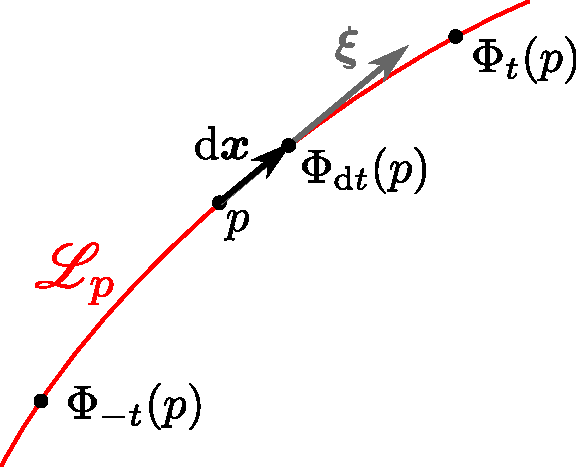
\includegraphics[height=0.25\textheight]{def_orbit_group.pdf}}
\caption[]{\label{f:neh:orbit_group} \footnotesize
Orbit of a point $p$ under the action $\Phi$ of a 1-dimensional Lie group, parameterized
by $t\in\R$. The vector $\w{\xi} = \D\w{x}/\D t$ is the group
generator associated with this parameter.}
\end{figure}

A 1-dimensional Lie group $G$ is said to be a
\defin{symmetry group}\index{symmetry!group}\index{group!symmetry --}
of the spacetime $(\M,\w{g})$ if there is an action $\Phi$ of $G$ on $\M$
such that for any value of the parameter $t$ of $G$,
$\Phi_t$ is an \defin{isometry}\index{isometry} of $(\M,\w{g})$, i.e. $\Phi_t$
preserves the ``distances'' and more generally the ``scalar products'' on
$(\M,\w{g})$, in the following sense: for any $p\in\M$ and any pair of points $(q,r)$
infinitely close to $p$, we shall have
\be \label{e:neh:isometry_dx}
    \left.\w{g}\right| _{\Phi_t(p)}(\D\w{x}', \D\w{y}') =
        \left.\w{g}\right| _{p}(\D\w{x}, \D\w{y}) ,
\ee
with the infinitesimal displacement vectors $\D\w{x} := \vp{pq}$, $\D\w{y} := \vp{pr}$,
$\D\w{x}' := \vp{\Phi_t(p)\Phi_t(q)}$ and $\D\w{y}' := \vp{\Phi_t(p)\Phi_t(r)}$
(cf. Sec.~\ref{s:fra:spacetime}).
Now, by definition, $\D\w{x}'$ is nothing but the pushforward
of the vector $\D\w{x}\in T_p\M$ to the tangent space
$T_{\Phi_t(p)}\M$ by the map $\Phi_t$
(cf. Sec.~\ref{s:bas:Lie_der_vector} of Appendix~\ref{s:bas}),
and similarly $\D\w{y}'$ is the pushforward of $\D\w{y}$ by $\Phi_t$:
\[
    \D\w{x}' = \Phi_t^*(\D\w{x}) \quad\mbox{and}\quad
    \D\w{y}' = \Phi_t^*(\D\w{y}) .
\]
By rescaling by infinitely small parameters (using the bilinearity of $\w{g}$),
it is clear that (\ref{e:neh:isometry_dx})
holds for finite vectors as well, so that we may say that $\Phi_t$ is an
isometry of $(\M,\w{g})$ iff
\be \label{e:neh:isometry}
    \forall p\in\M,\  \forall (\w{u},\w{v}) \in (T_p\M)^2,\quad
    \left. \w{g}\right| _{\Phi_t(p)} \left(\Phi_t^*\w{u}, \Phi_t^*\w{v}\right) =
    \left. \w{g}\right| _{p} (\w{u},\w{v}) ,
\ee
where $\Phi_t^* \w{u}$ (resp. $\Phi_t^* \w{v}$) is the pushforward of the vector $\w{u}\in T_p\M$ (resp. $\w{v}\in T_p\M$)
to the tangent space $T_{\Phi_t(p)}\M$ by $\Phi_t$ [cf. Eq.~(\ref{e:bas:def_Phi_eps})].
Given the definition (\ref{e:bas:def_pullback}) of the pullback of
a bilinear form, we may reexpress the isometry condition (\ref{e:neh:isometry})
in terms of the
pullback of $\w{g}$ by $\Phi_t$:
\be \label{e:neh:isometry_pullback}
    \Phi_t^*\w{g} = \w{g} .
\ee
According the definition (\ref{e:bas:def_Lie_der_covar}) of the Lie
derivative, we have
\be
    \Lie{\xi} \w{g} := \lim_{t \rightarrow 0} \frac{1}{t}
    \left( \Phi_t^*\w{g} - \w{g} \right) .
\ee
If $G$ is a symmetry group of $(\M,\w{g})$ with generator $\w{\xi}$,
the isometry condition
(\ref{e:neh:isometry_pullback}) leads then to
$\Lie{\xi}\w{g} = 0$. The reverse is true by integration. Hence
we conclude:
\begin{greybox}
A 1-dimensional Lie group $G$
is a symmetry group of the spacetime $(\M,\w{g})$ iff the Lie derivative
of the metric tensor along a generator $\w{\xi}$ of $G$
vanishes identically:
\be \label{e:neh:Lie_xi_g}
    \encadre{\Lie{\xi}\w{g} = 0 } .
\ee
The vector field $\w{\xi}$ is then called a \defin{Killing vector}\index{Killing!vector field}
of $(\M,\w{g})$.
\end{greybox}
Expressing the Lie derivative via Eq.~(\ref{e:bas:Lie_der_comp_nab}) of Appendix~\ref{s:bas},
we see immediately that Eq.~(\ref{e:neh:Lie_xi_g}) is equivalent to the so-called
\defin{Killing equation}\index{Killing!equation}:
\be \label{e:neh:Killing_equation}
    \encadre{ \nabla_\alpha \xi_\beta + \nabla_\beta \xi_\alpha = 0 }.
\ee

If terms of the components $g_{\alpha\beta}$ of $\w{g}$ with respect to
coordinates $(x^\alpha) = (t,x^1,\ldots,x^{n-1})$ adapted to the Killing vector $\w{\xi}$,
i.e. such that $\w{\xi} = \wpar_t$, the isometry condition (\ref{e:neh:Lie_xi_g})
is equivalent to
\be
    \der{g_{\alpha\beta}}{t} = 0 .
\ee
\begin{proof}
This is a direct consequence of the identity (\ref{e:bas:Lie_adapted}).
\end{proof}


\subsection{Definition and examples of Killing horizons} \label{s:neh:def_Killing_hor}

\begin{greybox}
A \defin{Killing horizon}\index{Killing!horizon}\index{horizon!Killing --} is
a null hypersurface $\Hor$ in a spacetime $(\M,\w{g})$ admitting a
Killing vector field $\w{\xi}$ such that, on $\Hor$, $\w{\xi}$ is
normal to $\Hor$.
\end{greybox}

Thus the existence of a Killing horizon requires that the spacetime $(\M,\w{g})$ has
some continuous symmetry
(usually stationarity), namely that it is invariant under the action of a
1-parameter group, as described in Sec.~\ref{s:neh:symmetries}.
A definition equivalent to the above one is then:
\begin{greybox}
A \defin{Killing horizon} is a null
hypersurface $\Hor$ whose null geodesic generators are orbits of a
1-parameter group of isometries of $(\M,\w{g})$.
\end{greybox}

\begin{remark}
The above definition implies that the Killing vector field $\w{\xi}$ is null
and non-vanishing on $\Hor$:
\be \label{s:neh:xi_on_KH}
    \left. \w{\xi}\cdot\w{\xi} \right| _{\Hor} = 0 \qquad\mbox{and}\qquad
    \left. \w{\xi} \right| _{\Hor} \not= 0 .
\ee
Indeed, if $\w{\xi}$ is vanishing at some point of $\Hor$, it cannot be
considered as a normal vector to $\Hor$.
\end{remark}

We shall see in Chap.~\ref{s:sta} that in a stationary spacetime, a black hole
event horizon must be a Killing horizon.

\begin{figure}
\centerline{\includegraphics[width=0.6\textwidth]{def_hplaneKilling-boost.pdf}}
\caption[]{\label{f:neh:hplaneKilling-boost} \footnotesize
Null half-hyperplanes $\Hor^+$ and $\Hor^-$ as Killing horizons for the
Killing vector field $\w{\xi}=x \wpar_t + t \wpar_x$ generating Lorentz boosts
in Minkowski spacetime. The green lines are the null geodesic generators of
$\Hor$, while the thick black line (actually a 2-plane) marks the location
where $\w{\xi}$ vanishes.}
\end{figure}

\begin{example}[null hyperplane as a translation-Killing horizon]
\label{x:neh:transKH}
Let us consider the null hyperplane of Minkowski spacetime $\Hor$ discussed in
Examples~\ref{x:def:null_hyp}, \ref{x:def:null_hyp2} and \ref{x:def:null_hyp3}
of Chap.~\ref{s:def}.
$\Hor$ is defined by the equation $t=x$. The vector field
\be
    \w{\xi} := \wpar_t + \wpar_x
\ee
is a Killing vector of Minkowski spacetime: $\w{\xi}$ is the generator of
translations in the direction $\wpar_t + \wpar_x$, and these translations constitute a
1-dimensional subgroup of the Poincaré group --- the symmetry group of Minkowski
spacetime. We note that $\w{\xi}$ coincides with the null vector $\wl$
defined by Eq.~(\ref{e:def:wl_null_hyperplane}). Since $\wl$ is
normal to $\Hor$, we conclude immediately that $\Hor$ is a Killing horizon
with respect to $\w{\xi}$.
\end{example}

\begin{example}[null hyperplane as a boost-Killing horizon]
\label{x:neh:boostKH}
Let us consider the same null hyperplane $\Hor$ as above, but
with another Killing vector of Minkowski spacetime:
\be \label{e:neh:boost-Killing}
    \w{\xi} := x \wpar_t + t \wpar_x .
\ee
This vector is indeed the
generator of the 1-parameter group of Lorentz boosts\index{boost} in the $(t,x)$ plane.
On $\Hor$ we have (cf. Fig.~\ref{f:neh:hplaneKilling-boost}):
\[
    \w{\xi} \equalH t (\wpar_t + \wpar_x) \equalH t \, \wl ,
\]
where $\wl$ is the null normal to $\Hor$ defined by
Eq.~(\ref{e:def:wl_null_hyperplane}) and the notation $\equalH$ means that the equality holds only on $\Hor$. We conclude that $\w{\xi}$ is a normal to
the null hypersurface $\Hor$ as soon as $t\not=0$. Therefore, we may split
$\Hor\setminus\{t=0\}$ in two open half-hyperplanes:
\be \label{e:neh:boost-Killing_hor}
    \Hor^+ := \{ p\in\Hor,\quad t(p) > 0 \} \quad\mbox{and}\quad
    \Hor^- := \{ p\in\Hor,\quad t(p) < 0 \} ,
\ee
so that each of them is a Killing horizon with
respect to $\w{\xi}$ (cf. Fig.~\ref{f:neh:hplaneKilling-boost}).
\end{example}

\begin{example}[null hyperplane as a null-rotation-Killing horizon]
\label{x:neh:nullrotKH}
Another example of Killing horizon is still provided by the null hyperplane
$\Hor$ considered above, but this time with the Killing vector
\be \label{e:neh:xi_null_rotation}
   \w{\xi} := y( \wpar_t + \wpar_x ) + (t-x)\wpar_y .
\ee
This vector is indeed the generator of
null rotations leaving the plane
$\mathrm{Span}(\wl,\wpar_z)$ strictly invariant (cf. e.g. Sec.~6.4.5 of
Ref.~\cite{Gourg13}), $\wl$ being the null normal of $\Hor$ defined by
Eq.~(\ref{e:def:wl_null_hyperplane}). These null rotations form a
1-dimensional subgroup of the Lorentz group, and thereby
a symmetry group of Minkowski spacetime. It is also immediate to check that
the vector defined by (\ref{e:neh:xi_null_rotation}) obeys
Killing equation (\ref{e:neh:Killing_equation}).
On $\Hor$, $t-x=0$, so that
(\ref{e:neh:xi_null_rotation}) reduces to
\[
    \w{\xi}  \equalH y ( \wpar_t + \wpar_x )  \equalH y \, \wl .
\]
It follows that $\w{\xi}$ is a null normal to $\Hor$ as soon as $y\not=0$.
We may then split $\Hor\setminus\{y=0\}$ in two open half-hyperplanes:
\[
    \Hor_1 := \{ p\in\Hor,\quad y(p) < 0 \} \quad\mbox{and}\quad
    \Hor_2 := \{ p\in\Hor,\quad y(p) > 0 \} ,
\]
each of them being a Killing horizon with
respect to $\w{\xi}$ (cf. Fig.~\ref{f:neh:hplaneKilling-nullrot}).
\end{example}

\begin{figure}
\centerline{\includegraphics[width=0.6\textwidth]{def_hplaneKilling-nullrot.pdf}}
\caption[]{\label{f:neh:hplaneKilling-nullrot} \footnotesize
Null half-hyperplanes $\Hor_1$ and $\Hor_2$ as Killing horizons for the
Killing vector field $\w{\xi}=y( \wpar_t + \wpar_x ) + (t-x)\wpar_y$
generating null rotations
in Minkowski spacetime. The green lines are the null geodesic generators of
$\Hor$, while the thick black line (actually a 2-plane) marks the location
where $\w{\xi}$ vanishes.}
\end{figure}

\begin{example}[light cone as a counter-example]
The future light cone introduced in Example~\ref{x:def:light_cone} of Chap.~\ref{s:def} is \emph{not} a
Killing horizon of Minkowski spacetime: it is invariant under the action
of the Lorentz group, but its null generators are not invariant
under the action of a single 1-dimensional subgroup of the Lorentz group.
Actually the future light cone is an example of a more general structure,
which Carter has termed a
\defin{local isometry horizon}\index{local!isometry horizon}\index{isometry!horizon}\index{horizon!local isometry --} \cite{Carte67,Carte69}: a null hypersurface that is invariant under
some group $G$ of isometries (here: the Lorentz group) and such that each null
geodesic generator is an orbit of some 1-dimensional subgroup of $G$,
this subgroup being not necessarily the same from one null generator to the next
(here: using Minkowskian spherical
coordinates $(t,r,\th,\ph)$,
the null geodesic generator through the point of coordinates $(1,1,\th_0,\ph_0)$
is the orbit of this point under the subgroup of boosts in the plane
$(\th,\ph) = (\th_0,\ph_0)$). A Killing horizon is a local isometry horizon
for which $\dim G = 1$.
\end{example}


\begin{example}[Schwarzschild horizon] \label{x:neh:Schwarz_KH}
Given the expression (\ref{e:def:wl_Schw_hor}) for the null normal $\wl$
of the family of hypersurfaces $\Hor_u$ and the fact that the Schwarzschild
horizon $\Hor$ is defined by $r=2m$, we have
\be \label{e:neh:wl_wpt_Schw_hor}
    \wl \equalH \wpar_t .
\ee
Now the vector field $\wpar_t$ is clearly a Killing vector of metric $\w{g}$
as given by (\ref{e:def:Schw_metric}), since none of the metric components
$g_{\alpha\beta}$ depends upon $t$. Hence (\ref{e:neh:wl_wpt_Schw_hor})
shows that the Schwarzschild horizon is a Killing horizon. By the way,
Eq.~(\ref{e:neh:wl_wpt_Schw_hor}) was our motivation for the choice of the
null normal $\wl$ performed in Example~\ref{x:def:Schw_hor2} of Chap.~\ref{s:def}.
\end{example}

\begin{hist}
The concept of Killing horizon has been introduced by Brandon Carter\index{Carter, B.} in
1966 \cite{Carte66,Carte67} and developed in an article published in
1969 \cite{Carte69}. The properties of Killing horizons have been
studied in detail by Robert H. Boyer\index{Boyer, R.H.},
in an article prepared posthumously from his notes
by J.~Ehlers and J.L.~Stachel and published in 1969 \cite{Boyer69},
leading to the concept of \emph{bifurcate Killing horizon}, to be discussed in
Sec.~\ref{s:sta:bifur_Killing_hor} (cf. the historical note on page~\pageref{h:sta:Boyer}).
\end{hist}

\subsection{Killing horizons as non-expanding horizons}

Let $\Hor$ be a Killing horizon with cross-sections that are closed manifolds,
i.e. the topology of $\Hor$ is (\ref{e:def:H_topology}). Let us select the null normal $\wl$
that coincides with the Killing vector $\w{\xi}$ on $\Hor$:
$\wl \equalH \w{\xi}$.
Equation~(\ref{e:neh:Lie_xi_g}) then implies:
\[
    \Lie{\el} \w{g} \equalH 0 .
\]
Let $\Sp$ be a cross-section of $\Hor$; since $\w{q}$ is the metric induced by $\w{g}$
on $\Sp$, we deduce immediately that
\[
    \Lie{\el} \w{q} = 0 .
\]
From the definition (\ref{e:def:Theta}), it follows that the expansion rate
tensor of $\Sp$ vanishes identically:
\be \label{e:neh:Theta_zero_KillingH}
   \encadre{ \w{\Theta} = 0 }.
\ee
In particular we have
\[
    \theta_{(\wl)} = 0 .
\]
We conclude that
\begin{greybox}
Any Killing horizon with closed-manifold cross-sections is a non-expanding horizon.
\end{greybox}
Moreover, (\ref{e:neh:Theta_zero_KillingH}) shows that $\w{\Theta}$ vanishes
for all Killing horizons, while to get the same result on a generic non-expanding
horizon, one has to assume that the null energy condition holds on $\Hor$.

\subsection{Expressions of the non-affinity coefficient}

Let $\kappa$ be the non-affinity coefficient
(cf. Sec.~\ref{s:def:geod_gener} and \ref{s:geo:gener_param})
of the null normal $\wl$ coinciding with the Killing vector $\w{\xi}$
on a Killing horizon $\Hor$. According to the definition
(\ref{e:def:wl_geod_kappa}), we have
\be \label{e:neh:xi_nab_xi_kappa}
    \wnab_{\w{\xi}}\, \w{\xi} \equalH \kappa \, \w{\xi} .
\ee
The metric dual of this relation is
$\xi^\mu \nabla_\mu \xi_\alpha \equalH \kappa \, \xi_\alpha$.
Using Killing equation (\ref{e:neh:Killing_equation}) under the form
$\nabla_\mu \xi_\alpha = - \nabla_\alpha \xi_\mu$, we get
\[
    \xi^\mu \nabla_\alpha \xi_\mu \equalH - \kappa \, \xi_\alpha .
\]
Now $\xi^\mu \nabla_\alpha \xi_\mu = 1/2 \, \nabla_\alpha (\xi_\mu \xi^\mu)$.
Hence
\be
    \nabla_\alpha (\xi_\mu \xi^\mu) \equalH - 2 \kappa \, \xi_\alpha.
\ee
Since $\xi_\mu \xi^\mu = \w{\xi}\cdot\w{\xi}$ is a scalar field, we may
replace the covariant derivative by the differential:
\be \label{e:neh:dxi2_kappa}
    \encadre{ \dd (\w{\xi}\cdot\w{\xi}) \equalH - 2 \kappa \, \uu{\xi} } .
\ee

Another interesting relation is obtained from the Frobenius theorem\index{Frobenius!theorem}
applied to $\w{\xi}$. Indeed, since on $\Hor$, $\w{\xi}$ is normal to a hypersurface
($\Hor$), the Frobenius theorem in its dual formulation
(see e.g.
Theorem B.3.2 in Wald's textbook \cite{Wald84} or Theorem C.2 in
Straumann's textbook \cite{Strau13}) states that there exists a 1-form
$\w{a}$ such that
\be
    \dd \uu{\xi} \equalH \w{a} \wedge \uu{\xi} ,
\ee
or equivalently
\be \label{e:neh:Frobenius_xi}
  \nabla_\alpha \xi_\beta - \nabla_\beta \xi_\alpha \equalH
  a_\alpha \, \xi_\beta -  a_\beta  \, \xi_\alpha  .
\ee

\begin{remark}
In the case of the vector $\wl$, which is normal to $\Hor$ by definition,
the Frobenius identity is
Eq.~(\ref{e:def:ext_der_wl_comp}): $\nabla_\alpha \el_\beta - \nabla_\beta \el_\alpha =
  \nabla_\alpha \rho \, \el_\beta -  \nabla_\beta \rho \, \el_\alpha$.
Since $\wl \equalH \w{\xi}$, we may write
\[
  \nabla_\alpha \el_\beta - \nabla_\beta \el_\alpha \equalH
  \nabla_\alpha \rho \, \xi_\beta -  \nabla_\beta \rho \, \xi_\alpha .
\]
But in general,  $\nabla_\alpha \el_\beta \not= \nabla_\alpha \xi_\beta$ on $\Hor$,
since $\wl$ and $\w{\xi}$ do not coincide outside $\Hor$. Accordingly, one
cannot identify the left-hand side of the above equation with the left-hand side
of Eq.~(\ref{e:neh:Frobenius_xi}), so that the 1-form $\w{a}$ is \emph{not} $\wnab\rho$.
\end{remark}

Thanks to the Killing equation (\ref{e:neh:Killing_equation}), we may reshape
(\ref{e:neh:Frobenius_xi}) to
\be \label{e:neh:Frobenius_xi_Killing}
    2 \nabla_\alpha \xi_\beta \equalH
  a_\alpha \, \xi_\beta -  a_\beta \, \xi_\alpha  .
\ee
Contracting this relation with $\w{\xi}$, we get
\[
   2 \xi^\mu \nabla_\mu \xi_\alpha \equalH a_\mu \xi^\mu  \, \xi_\alpha
    -  \underbrace{\xi_\mu \xi^\mu}_{\equalH 0} \, a_\alpha .
\]
In view of Eq.~(\ref{e:neh:xi_nab_xi_kappa}), the left-hand side of this
equation is $2\kappa \xi_\alpha$. Hence we obtain
\be \label{e:neh:a_xi_2_kappa}
    a_\mu \xi^\mu \equalH 2 \kappa .
\ee
Besides, taking the square of (\ref{e:neh:Frobenius_xi_Killing}) leads to
\bea
    4 \nabla_\mu \xi_\nu \, \nabla^\mu \xi^\nu & \equalH &
        \left( a_\mu \xi_\nu -  a_\nu \xi_\mu \right)
       \left( a^\mu \xi^\nu - a^\nu \xi^\mu \right)
       \nonumber \\
       & \equalH & a_\mu a^\mu
        \underbrace{ \xi_\nu \xi^\nu}_{\equalH 0}
        - \underbrace{a_\mu \xi^\mu}_{2\kappa}
         \underbrace{a_\nu \xi^\nu}_{2\kappa}
        - \underbrace{a_\nu \xi^\nu}_{2\kappa}
            \underbrace{a_\mu \xi^\mu}_{2\kappa}
        + a_\nu  a^\nu
        \underbrace{ \xi_\mu \xi^\mu}_{\equalH 0}
         \nonumber \\
         & \equalH & - 8 \kappa^2 , \nonumber
\eea
where we have used Eq.~(\ref{e:neh:a_xi_2_kappa}).
Hence
\be \label{e:neh:kappa2}
    \encadre{\kappa^2 \equalH - \frac{1}{2}
        \nabla_\mu \xi_\nu \nabla^\mu \xi^\nu } .
\ee
This is an explicit expression of $\kappa$ in terms of the Killing vector
field $\w{\xi}$.
However, in actual calculations, it is generally preferable to employ
(\ref{e:neh:dxi2_kappa}) for evaluating $\kappa$, because the latter does not involve
the computation of any covariant derivative, contrary to (\ref{e:neh:kappa2}).


\subsection{The zeroth law of black hole mechanics} \label{s:neh:zeroth_law}

We are going to derive a result of great importance for black hole physics,
namely the non-affinity coefficient $\kappa$ discussed above
is constant on a Killing horizon, provided some mild energy condition holds.

Let us denote by $\wl$ the null normal to $\Hor$ that coincides with
the Killing vector field: $\wl \equalH \w{\xi}$. The vector field
$\wl$ is then a symmetry generator on $\Hor$, which implies
\be
    \Lie{\el} \kappa = 0 .
\ee
This means that $\kappa$ is constant along the field lines of $\wl$ (i.e. the
null geodesic generators of $\Hor$). It could however vary from a field line to another
one. To show that this is not the case, let us consider a cross-section
$\Sp$ of $\Hor$ and project the contracted Ricci identity (\ref{e:def:contract_Ricci_ident})
onto it, via the orthogonal projector $\vw{q}$ introduced in
Sec.~\ref{s:def:spacelike_sections}:
\[
    \nabla_\mu \Theta^\mu_{\ \, \nu} q^\nu_{\ \, \alpha} + \el^\mu \nabla_\mu \omega_\nu q^\nu_{\ \, \alpha}
       - \nabla_\nu \left( \theta_{(\wl)} + \kappa \right) q^\nu_{\ \, \alpha}
        + \left( \theta_{(\wl)} + \kappa \right) \omega_\nu q^\nu_{\ \, \alpha}
        - \Theta_{\alpha\mu} k^\nu \nabla_\nu \el^\mu \nonumber \\
     = R_{\mu\nu} \el^\mu q^\nu_{\ \, \alpha}, \nonumber
\]
where we have used $\Theta_{\nu\mu}  q^\nu_{\ \, \alpha} = \Theta_{\alpha\mu}$
and $\el_\nu q^\nu_{\ \, \alpha} = 0$.
Now, since $\Hor$ is a Killing horizon, we have $\w{\Theta}=0$ [cf. Eq.~(\ref{e:neh:Theta_zero_KillingH})] and in particular
$\theta_{(\wl)} =0$. Accordingly, the above equation reduces to
\be \label{e:neh:zeroth_law_step1}
    \el^\mu \nabla_\mu \omega_\nu q^\nu_{\ \, \alpha} - \nabla_\nu \kappa \, q^\nu_{\ \, \alpha}
    + \kappa  \, \omega_\nu q^\nu_{\ \, \alpha} = R_{\mu\nu} \el^\mu q^\nu_{\ \, \alpha} .
\ee
Let us express $\el^\mu \nabla_\mu \omega_\nu$ in terms of the Lie derivative
of $\w{\omega}$ along $\wl$ via formula (\ref{e:bas:Lie_der_comp_nab}) of Appendix~\ref{s:bas}:
\be \label{e:neh:nab_l_omega_prov}
    \el^\mu \nabla_\mu \omega_\nu q^\nu_{\ \, \alpha} = \left( \Liec{\el}\omega_\nu - \omega_\mu \nabla_\nu \el^\mu \right) q^\nu_{\ \, \alpha} .
\ee
Now, since $\wl$ is a symmetry generator on $\Hor$, we have
\be \label{e:neh:Lie_l_Homeg_zero}
    \Lie{\el} {}^{\Hor}\!\w{\omega} = 0 ,
\ee
where ${}^{\Hor}\!\w{\omega}$ is the restriction of $\w{\omega}$ to vectors
tangent to $\Hor$, which has been shown to be a geometric quantity intrinsic to
$\Hor$ and $\wl$ in Sec.~\ref{e:neh:induced_connection} and therefore has to
obey the spacetime symmetry generated by $\w{\xi} \equalH \wl$.
Any vector field $\w{v}$ defined on $\Hor$ but not necessarily tangent to $\Hor$ can
be split in a unique way into a part tangent to $\Hor$, $\w{v}^\parallel$ say,
and a part along the transverse null vector field $\w{k}$ according
to\footnote{$\w{v}^\parallel = \w{\Pi}(\w{v})$, where $\w{\Pi}$ is the
the projector onto $\Hor$ along $\w{k}$, as expressed by Eq.~(\ref{e:def:def_proj_H_along_k}).}
\[
     \w{v} = \w{v}^\parallel - \langle \uu{\ell}, \w{v} \rangle \w{k} ,
\]
so that
\[
    \langle\Lie{\el}\w{\omega}, \w{v} \rangle =
    \langle\Lie{\el}\w{\omega}, \w{v}^\parallel \rangle
    -  \langle \uu{\ell}, \w{v} \rangle  \langle\Lie{\el}\w{\omega}, \w{k} \rangle .
\]
The first term in the right-hand side vanishes as a consequence of
(\ref{e:neh:Lie_l_Homeg_zero}); indeed,
the Leibniz rule allows us to write
\[
    \langle \Lie{\el}\w{\omega}, \w{v}^\parallel  \rangle =
    \Lie{\el} \langle \w{\omega}, \w{v}^\parallel  \rangle - \langle \w{\omega}, \Lie{\el}\w{v}^\parallel  \rangle
    =  \Lie{\el} \langle {}^{\Hor}\!\w{\omega}, \w{v}^\parallel  \rangle - \langle {}^{\Hor}\!\w{\omega}, \Lie{\el}\w{v}^\parallel  \rangle
    = \langle \underbrace{\Lie{\el}{}^{\Hor}\!\w{\omega}}_{0}, \w{v}^\parallel  \rangle = 0 ,
\]
where the second equality follows from the fact that $\Lie{\el}\w{v}^\parallel $ is a vector field tangent to $\Hor$ by the very definition of a Lie derivative (cf. Sec.~\ref{s:bas:Lie}), $\wl$ being tangent to $\Hor$.
Hence the symmetry property (\ref{e:neh:Lie_l_Homeg_zero}) translates to
the Lie derivative of $\w{\omega}$ along $\wl$ being proportional to the
1-form $\uu{\ell}$:
\be
    \Lie{\el}\w{\omega} = - \langle\Lie{\el}\w{\omega}, \w{k} \rangle \, \uu{\ell} .
\ee
Using this formula into Eq.~(\ref{e:neh:nab_l_omega_prov}) leads to
\[
       \el^\mu \nabla_\mu \omega_\nu q^\nu_{\ \, \alpha} =
       - k^\mu \Liec{\el} \omega_\mu  \underbrace{\ell_\nu q^\nu_{\ \, \alpha}}_{0}
       - \omega_\mu \nabla_\nu \el^\mu  q^\nu_{\ \, \alpha}
       = - \omega_\mu \nabla_\nu \el^\mu  q^\nu_{\ \, \alpha}  .
\]
Accordingly, Eq.~(\ref{e:neh:zeroth_law_step1}) becomes successively
\bea
   & & - \omega_\mu \nabla_\nu \el^\mu  q^\nu_{\ \, \alpha}
     - \nabla_\nu \kappa \, q^\nu_{\ \, \alpha}
    + \kappa  \, \omega_\nu q^\nu_{\ \, \alpha} = R_{\mu\nu} \el^\mu q^\nu_{\ \, \alpha} \nonumber \\
   & &  - \omega_\mu \left(\Theta_\nu^{\ \, \mu}
        + \omega_\nu \el^\mu - \el_\nu k^\sigma \nabla_\sigma \el^\mu \right) q^\nu_{\ \, \alpha}
     - \nabla_\nu \kappa \, q^\nu_{\ \, \alpha}
    + \kappa  \, \omega_\nu q^\nu_{\ \, \alpha} = R_{\mu\nu} \el^\mu q^\nu_{\ \, \alpha} \nonumber \\
   & &   - \omega_\mu
   \underbrace{\Theta_\alpha^{\ \, \mu}}_{0}
        - \underbrace{\omega_\mu \el^\mu}_{\kappa} \omega_\nu q^\nu_{\ \, \alpha}
     - \nabla_\nu \kappa \, q^\nu_{\ \, \alpha}
    + \kappa  \, \omega_\nu q^\nu_{\ \, \alpha} = R_{\mu\nu} \el^\mu q^\nu_{\ \, \alpha}  \nonumber \\
   & &
   - \nabla_\nu \kappa \, q^\nu_{\ \, \alpha} = R_{\mu\nu} \el^\mu q^\nu_{\ \, \alpha} , \nonumber
\eea
where we have used (\ref{e:def:nab_l_Theta}) to get the second line,
the identity
$\el_\nu q^\nu_{\ \, \alpha} = 0$ to get the third one and
(\ref{e:def:omega_l_kappa}) to substitute $\kappa$ for
$\omega_\mu \el^\mu$.
In the above equation appears the covariant derivative of $\kappa$ along $\Sp$,
which we denote by $\DS$:
\be
    \DSc_\alpha \kappa := \nabla_\nu \kappa \, q^\nu_{\ \, \alpha} .
\ee
Using the Einstein equation (\ref{e:fra:Einstein_eq_n}), we may then rewrite
the above relation as
\[
    \DSc_\alpha \kappa = -  \frac{2}{n-2}\,\Lambda\,
    \underbrace{g_{\mu\nu}  \el^\mu q^\nu_{\ \, \alpha}}_{\el^\mu q_{\mu\alpha} = 0}
    - 8\pi \Big( T_{\mu\nu} \el^\mu q^\nu_{\ \, \alpha}
    - \frac{1}{n-2}\,  T \, \underbrace{g_{\mu\nu}  \el^\mu q^\nu_{\ \, \alpha}}_{\el^\mu q_{\mu\alpha} = 0} \Big) ,
\]
i.e.
\be \label{e:neh:DS_kappa_W}
    \DSc_\alpha \kappa = - 8\pi T_{\mu\nu} \el^\mu q^\nu_{\ \, \alpha} .
\ee
To go further, we shall assume that matter and the non-gravitational fields
obey the
\defin{null dominant energy condition}\index{null!dominant energy condition}\index{energy!condition!null dominant--}:
\be
   \begin{array}{ll}
    \w{W} := - \vw{T}(\wl, .) \ & \mbox{is future-directed null or timelike} \\
    & \mbox{for any future-directed null vector $\wl$} .
    \end{array}
\ee
In the above equation, $\vw{T}(\wl, .)$ stands for the vector field
that is the metric dual of the 1-form $\w{T}(\wl, .)$; in index notation,
\[
    W^\alpha = - g^{\alpha\nu} T_{\mu\nu}\el^\mu = - T_\mu^{\ \, \alpha} \el^\mu .
\]
Note that the null dominant energy condition implies the null energy condition
discussed in Sec.~\ref{s:neh:NEH_Theta_zero}, since
\[
    \w{T}(\wl, \wl) = - \w{W}\cdot\wl \geq 0 ,
\]
the inequality holding because both $\w{W}$ and $\wl$ are future-directed.

The null dominant energy condition is implied by continuity by the
\defin{dominant energy condition}\index{dominant energy condition}\index{energy!condition!dominant--}:
\be
   \begin{array}{ll}
    \w{W} := - \vw{T}(\w{u}, .) \ & \mbox{is future-directed null or timelike} \\
    & \mbox{for any future-directed timelike vector $\w{u}$} .
    \end{array}
\ee
Physically, the dominant energy condition states that, with respect to any
observer (represented by its 4-velocity $\w{u}$, which is future-directed timelike),
the energy of matter and non-gravitational fields, moves at a speed
at most equal to $c$.

We note that in the right-hand side of (\ref{e:neh:DS_kappa_W}), there appears the
orthogonal projection of $\w{W}$ onto $\Sp$ (more precisely its metric dual).
If we assume the null dominant energy condition, the null energy condition
holds and we have, according to (\ref{e:neh:T_l_l_zero}),
\[
    \wl \cdot \w{W} = - \w{T}(\wl, \wl) = 0 ,
\]
This implies that the vector $\w{W}$ is tangent to $\Hor$. The latter
being a null hypersurface, $\w{W}$ must then be
either collinear to $\wl$ or spacelike (cf. the lemma in Sec.~\ref{s:def:spacelike_sections}).
Now, according to the null dominant energy condition, $\w{W}$ cannot be
spacelike. We conclude that $\w{W}$ is collinear to $\wl$. Consequently its
orthogonal projection onto $\Sp$ is zero:
\[
    q^\alpha_{\ \, \nu} W^\nu = - q^\alpha_{\ \, \nu} T_\mu^{\ \, \nu} \el^\mu = 0 .
\]
Hence the right-hand side of (\ref{e:neh:DS_kappa_W}) vanishes identically
and we are left with
\[
    \DSc_\alpha \kappa = 0 .
\]
This means that $\kappa$ is constant over $\Sp$. Given that $\kappa$ is
constant along each null geodesic generator of $\Hor$, this completes the demonstration
that $\kappa$ is constant over $\Hor$. More precisely, we have shown that
\begin{greybox}
If matter and non-gravitational fields obey the null dominant energy condition
on the Killing horizon $\Hor$, then the non-affinity coefficient $\kappa$
of the null normal coinciding with the Killing vector field on
$\Hor$ is constant over $\Hor$:
\be \label{e:neh:zeroth_law}
    \encadre{\kappa = \mathrm{const}.}
\ee
\end{greybox}
In the context of Killing horizons, the non-affinity coefficient $\kappa$ is
called the horizon's \defin{surface gravity}\index{surface!gravity},
for a reason to be detailed in Sec.~\ref{s:neh:surface_gravity},
and the result
(\ref{e:neh:zeroth_law}) is known as the
\defin{zeroth law of black hole mechanics}\index{zeroth law}. More precisely,
the latter states that the surface gravity of a black hole in equilibrium is
constant and we shall see in Chap.~\ref{s:sta} that the event horizon of a black hole in
equilibrium is a Killing horizon.

\begin{example}[null hyperplane as a translation-Killing horizon]
\label{x:neh:transKH_kappa}
For the null hyperplane $\Hor$ considered in Example~\ref{x:neh:transKH} as a Killing horizon with respect to the translation group along its normal, we have
$\kappa = 0$, as already noticed in Example~\ref{x:def:null_hyp3} of Chap.~\ref{s:def}
[Eq.~(\ref{e:def:kappa_0_nullhyp})], which is obviously constant over $\Hor$.
\end{example}

\begin{example}[null hyperplane as a boost-Killing horizon]
\label{x:neh:boostKH_kappa}
Let us consider each of the null half-hyperplanes $\Hor^+$
and $\Hor^-$ of Example~\ref{x:neh:boostKH}, which are Killing horizons with
respect to the boost Killing vector $\w{\xi} = x \wpar_t + t \wpar_x$. On
$\Hor^+$, the future-directed null normal coinciding with this Killing vector
is $\wl^+ = t\,  \wl$, $\wl$ being the geodesic null normal defined by
$\wl:= \wpar_t + \wpar_x$ [cf. Eq.~(\ref{e:def:wl_null_hyperplane})].
Using $\kappa_{\wl} = 0$ and the scaling law (\ref{e:def:rescale_kappa}),
we get the non-affinity
coefficient of $\wl^+$ as $\kappa_+= \wnab_{\wl} t = \partial_t t + \partial_x t$, i.e.
\[
    \kappa_+ = 1 .
\]
On $\Hor^-$, $\w{\xi}$ is past-directed (cf. Fig.~\ref{f:neh:hplaneKilling-boost}).
Sticking to future-directed null normals, we shall then consider $\Hor^-$
as a Killing horizon with respect to the Killing vector field $-\w{\xi}$.
The future-directed null normal coinciding with $-\w{\xi}$ on $\Hor^-$ is then
$\wl^- = -t\,  \wl$, from which we deduce the non-affinity
coefficient of $\wl^-$: $\kappa_-= \wnab_{\wl} (-t) = \partial_t (-t) + \partial_x (-t)$, i.e.
\[
    \kappa_- = -1 .
\]
We check that $\kappa_+$ (resp.  $\kappa_-$) is constant over the Killing horizon $\Hor^+$ (resp. $\Hor^-$), in agreement with the result above.
\end{example}

\begin{example}[null hyperplane as a null-rotation-Killing horizon]
\label{x:neh:nullrotKH_kappa}
In Example~\ref{x:neh:nullrotKH}, we have introduced the Killing horizons
$\Hor_1$ and $\Hor_2$ with respect to the null-rotation Killing vector
$\w{\xi} = y( \wpar_t + \wpar_x ) + (t-x)\wpar_y$ of Minkowski spacetime.
On $\Hor_1$, $\w{\xi}$ is past-directed (cf. Fig.~\ref{f:neh:hplaneKilling-nullrot}),
so that we shall actually consider $\Hor_1$
as a Killing horizon with respect to the Killing vector field $-\w{\xi}$.
The future-directed null normal coinciding with $-\w{\xi}$ on $\Hor_1$ is then
$\wl_1 = - y\, \wl$. Since it is clearly constant along the null geodesic generators
of $\Hor_1$, we have $\wnab_{\wl_1}\wl_1 = 0$, hence the
associated non-affinity coefficient vanishes:
\[
    \kappa_1 = 0 .
\]
On $\Hor_2$, $\w{\xi}$ is future-directed (cf. Fig.~\ref{f:neh:hplaneKilling-nullrot})
and the null normal coinciding with it is $\wl_2 =  y\,  \wl$, whose non-affinity
coefficient is
\[
    \kappa_2 = 0 .
\]
\end{example}

\begin{example}[Schwarzschild and Kerr horizons]
\label{x:neh:Schw_Kerr_kappa}
We have found in Example~\ref{x:def:Schw_hor3} of Chap.~\ref{s:def} [cf. Eq.~(\ref{e:def:kappa_Schw_hor})]
that on a Schwarzschild horizon:
\[
  \kappa = \frac{1}{4m},
\]
which is clearly constant. But
this last feature is rather trivial since the Schwarzschild horizon is spherically
symmetric, so that no dependence of $\kappa$ on $\th$ nor $\ph$ could have been expected.
A much less trivial example is that of the event horizon of a Kerr black hole,
which we shall discuss in Chap.~\ref{s:ker}. This horizon is only axisymmetric,
so that a priori $\kappa$ could depend on $\th$. But it does not, as we shall
see in Sec.~\ref{s:ker:surf_grav}:
\[
    \kappa = \frac{\sqrt{m^2 - a^2}}{2m(m + \sqrt{m^2-a^2})} ,
\]
where $(m,a)$ are the two constant parameters of the Kerr solution. Note that for $a=0$,
we recover the Schwarzschild value: $\kappa= 1/(4m)$.
\end{example}

\begin{hist}
The constancy of $\kappa$ for a Killing horizon has been proven by Stephen Hawking\index{Hawking, S.W.}
in his lecture at the famous Les Houches School of Summer 1972 \cite{Hawki73} (p.~43).
It has also been proven without requiring the dominant energy condition, but
assuming axisymmetry by Brandon Carter\index{Carter, B.} in his lecture at the same Les Houches School
\cite{Carte73b} (Theorem 8, p.~167).
A third proof of the constancy of $\kappa$ using the dominant energy condition
has also been given in 1973 by James Bardeen\index{Bardeen, J.M.}, Brandon Carter and
Stephen Hawking
in their seminal article \emph{The Four Laws of Black Hole Mechanics}
\cite{BardeCH73}.
\end{hist}

\subsection{Classification of Killing horizons} \label{s:neh:classif_KH}

Since $\kappa$ is constant on $\Hor$ (assuming the dominant
energy condition), we may use it to classify Killing horizons in two
categories, depending whether $\kappa$ vanishes or not:
\begin{itemize}
\item if $\kappa = 0$, the Killing vector $\w{\xi}$ is then a geodesic vector on $\Hor$
and $\Hor$ is called a \defin{degenerate Killing horizon}\index{degenerate!Killing horizon}\index{Killing!horizon!degenerate --};
\item if $\kappa \not=0$, $\w{\xi}$ is only a pregeodesic vector on $\Hor$
(cf. Sec.~\ref{s:geo:gener_param})
and $\Hor$ is called a \defin{non-degenerate Killing horizon}\index{non-degenerate!Killing horizon}\index{Killing!horizon!non-degenerate --}.
\end{itemize}

\begin{example}[Killing horizons in Minkowski spacetime]
In Minkowski spacetime, the null hyperplane as a translation-Killing horizon
(Example~\ref{x:neh:transKH_kappa}) and the two half-hyperplanes as
null-rotation-Killing horizons (Example~\ref{x:neh:nullrotKH_kappa}) are
degenerate Killing horizons, while the two half-hyperplanes as
boost-Killing horizons (Example~\ref{x:neh:boostKH_kappa}) are non-degenerate.
\end{example}

\begin{example}[Schwarzschild and Kerr horizons]
From the values of $\kappa$ given in Example~\ref{x:neh:Schw_Kerr_kappa},
we see that the Schwarzschild horizon and the Kerr horizon for
$a<m$ are non-degenerate Killing horizons, while the Kerr horizon for
$a=m$ is a degenerate one.
\end{example}

The next example regards the anti-de Sitter spacetime and will play some
role in the study of the extremal ($a=m$) Kerr black hole in Chap.~\ref{s:exk}.

\begin{figure}
\centerline{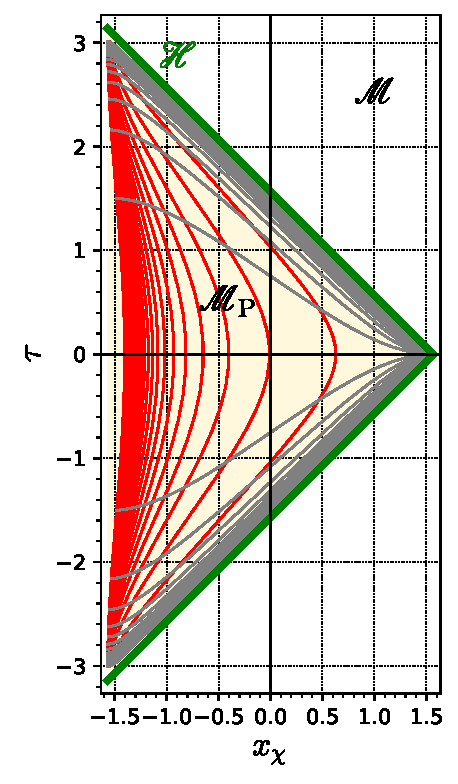
\includegraphics[width=0.4\textwidth]{neh_AdS_Poincare_patch.pdf}\ \qquad \
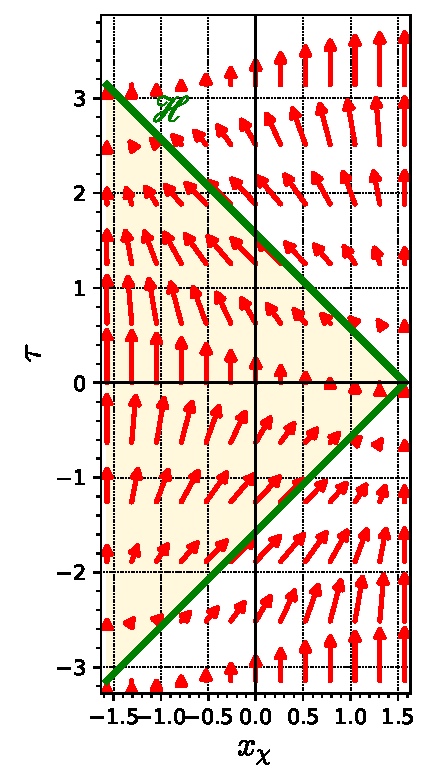
\includegraphics[width=0.4\textwidth]{neh_AdS_Killing_vec.pdf}
}
\caption[]{\label{f:neh:AdS_example} \footnotesize
\emph{Left:} 2-dimensional slice $(x,y)=(0,0)$ of the Poincaré patch $\M_{\rm P}$ of anti-de Sitter spacetime plotted in terms of the (global) coordinates $\tau$ and
$x_\chi := \chi \cos\ph$ (pale yellow region). From Eq.~(\ref{e:neh:Poincare_coord}),
$(x,y)=(0,0)$ implies $\th=\pi/2$ and $\ph=0$ or $\pi$, so that $x_\chi = \chi$
in the right half of the plot ($\ph=0$) and $x_\chi = - \chi$ in the left half
($\ph=\pi$). The plotted slice of $\M_{\rm P}$ is thus spanned by the
Poincaré coordinates $(t,u)$.
The red lines are curves of constant $u$, i.e. integral curves of
the coordinate vector field $\wpar_t = \w{\xi}$, with $u$ increasing from $0$ to $+\infty$
from the right to the left of the diagram. The grey lines are
curves of curves
of constant $t$, i.e. integral curves of the coordinate vector field $\wpar_u$,
with $t$ increasing from $-\infty$ to $+\infty$ from the bottom to the top
of the diagram. The Poincaré horizon $\Hor$ is depicted in green.
Each connected component of $\Hor$ appears as a straight line segment, since for $\th=\pi/2$
and $\ph\in\{0,\pi\}$, $u = 0 \iff \cos\tau = \pm \sin\chi$ ($+$ for $\ph=0$ and $-$ for $\ph=\pi$).
Note that the curves of constant $u$ tend to $\Hor$ when $u\to 0$, in agreement
with the characterization of $\Hor$ by $u=0$. The curves of constant
$t$ tend to $\Hor$ when $t\to \pm\infty$, which is expected as well since
the first line of Eq.~(\ref{e:neh:Poincare_coord}) and Eq.~(\ref{e:neh:AdS:def_u})
imply that $u\to 0$ for $t\to \pm\infty$.
\emph{Right:} Killing vector field $\w{\xi}$ defined by Eq.~(\ref{e:neh:AdS:def_xi})
on AdS$_{4}$; $\w{\xi}$ is timelike everywhere, except on the Poincaré
horizon $\Hor$, where it is null (and normal, and thus tangent, to $\Hor$).
\textsl{[Figures generated by the notebook \ref{s:sam:Poincare_hor}]}
}
\end{figure}

\begin{example}[Poincaré horizon in AdS$_{4}$] \label{x:neh:AdS}
The 4-dimensional \defin{anti-de Sitter spacetime}\index{anti-de Sitter spacetime} (AdS$_{4}$)
is $(\M,\w{g})$ with $\M\simeq \mathbb{R}^4$ and $\w{g}$ is the metric
whose components in the so-called \emph{global static coordinates}
$(\tau,r,\th,\ph)$ are given by
\be \label{e:neh:AdS4}
    \w{g} = \ell^2 \left[ - (1 + r^2) \, \dd \tau^2
    + \frac{\dd r^2}{1 + r^2} + r^2 \left( \dd\th^2 + \sin^2\th \, \dd\ph^2 \right) \right] ,
\ee
where $\ell$ is a positive constant.
Note that $\tau$ spans $\mathbb{R}$, $r$ spans $(0,+\infty)$,
while $(\th,\ph)$ are standard spherical coordinates on $\mathbb{S}^2$:
$\th\in(0,\pi)$ and $\ph\in(0,2\pi)$.
The metric (\ref{e:neh:AdS4}) is a solution
of the Einstein equation (\ref{e:fra:Einstein_eq}) with
the negative cosmological constant $\Lambda = - 3/\ell^2$
and $\w{T}=0$ (vacuum). Using the so-called \emph{conformal coordinates} $(\tau,\chi,\th,\ph)$ with
$\chi := \arctan r \in (0,\pi/2)$, one gets
\be \label{e:neh:metrix_AdS_conformal}
   \w{g} = \frac{\ell^2}{\cos^2\chi} \left[ - \dd \tau^2
    + \dd \chi^2 + \sin^2\chi \left( \dd\th^2 + \sin^2\th \, \dd\ph^2 \right) \right] .
\ee
Note that $(\chi,\th,\ph)$ spans one half\footnote{It would span the whole hypersphere if
$\chi$ would run in all of $(0,\pi)$, instead of being limited to $(0,\pi/2)$.} of the hypersphere\index{hypersphere} $\mathbb{S}^3$.
Yet another set of coordinates commonly used in AdS$_{4}$ is \defin{Poincaré coordinates}\index{Poincaré!coordinates on AdS$_n$} $(t,x,y,u)$. They cover only a subpart
$\M_{\rm P}$ of $\M$ (cf. Fig.~\ref{f:neh:AdS_example}), usually called the \defin{Poincaré patch}\index{Poincaré!patch!of AdS$_4$} and defined by
\be \label{e:neh:def_Poincare_patch}
    \M_{\rm P}:\quad u > 0 \qand -\pi < \tau < \pi,
\ee
where $u$ is the following scalar field on $\M$:
\be \label{e:neh:AdS:def_u}
    u :=  \frac{\ell (\cos\tau - \sin\chi\sin\th\cos\ph)}{\cos\chi} .
\ee
On $\M_{\rm P}$, the Poincaré coordinates $(t,x,y,u)$ are related to the conformal coordinates
$(\tau,\chi,\th,\ph)$ by\footnote{See e.g. Ref.~\cite{BayonB07}.}
\be \label{e:neh:Poincare_coord}
    \left\{ \begin{array}{l}
    t = \frac{\ell \sin\tau}{\cos\tau - \sin\chi\sin\th\cos\ph} \\[1ex]
    x = \frac{\ell \sin\chi\sin\th\sin\ph}{\cos\tau - \sin\chi\sin\th\cos\ph} \\[1ex]
    y = \frac{\ell \sin\chi\cos\th}{\cos\tau - \sin\chi\sin\th\cos\ph} \\[1ex]
    u = \frac{\ell (\cos\tau - \sin\chi\sin\th\cos\ph)}{\cos\chi} .
    \end{array}\right.
\ee
The last line is simply (\ref{e:neh:AdS:def_u}) restricted to $\M_{\rm P}$, the scalar field $u$
being viewed there as one of the Poincaré coordinates.
The metric components with respect to Poincaré coordinates\footnote{The name \emph{Poincaré coordinates} stems from a variant of these coordinates obtained by using
$z:=\ell^2/u$ instead of $u$, so that
$\w{g} = \ell^2 \left( - \dd t^2 + \dd x^2 + \dd y^2 + \dd z^2 \right)/z^2$,
which is similar to the metric of the Poincaré half-space\index{Poincaré!half-space} model of
the hyperbolic space $\mathbb{H}^4$, except for the signature $(-,+,+,+)$
instead of $(+,+,+,+)$.}
are (cf. the notebook~\ref{s:sam:Poincare_hor} for the computation):
\be \label{e:neh:AdS:metric_Poincare}
   \w{g} = \frac{u^2}{\ell^2} \left( - \dd t^2 + \dd x^2 + \dd y^2 \right)
   + \frac{\ell^2}{u^2} \, \dd u^2 .
\ee
The \defin{Poincaré horizon}\index{Poincaré!horizon of AdS$_4$}
is the hypersurface $\Hor$ bounding the Poincaré patch $\M_{\rm P}$ in $\M$. In view of the definition
(\ref{e:neh:def_Poincare_patch}) of the latter, $\Hor$ appears to be the level set $u=0$:
\be \label{e:neh:def_Poincare_hor}
    \Hor:\quad u = 0 \qand -\pi < \tau < \pi,
\ee
Note that $\Hor$ is not included in $\M_{\rm P}$, so that the Poincaré coordinates are not
defined on $\Hor$ (except for $u$, they actually diverge in the vicinity of $\Hor$).
Note also that $\Hor$ has two connected components, one with
$\tau \in (-\pi,0)$ and the other one with $\tau \in (0,\pi)$, since $u=0$
cannot be achieved for $\tau=0$, as a consequence of
formula~(\ref{e:neh:AdS:def_u}) and $|\sin\chi|<1$ on $\M$.
The Poincaré horizon is depicted in Fig.~\ref{f:neh:AdS_example}.
Its normal is given by the gradient of $u$, so that the vector field
defined in all $\M$ by
$\w{k} := \vec{\wnab} u$ is normal
to $\Hor$ on $\Hor$.
Given expressions (\ref{e:neh:metrix_AdS_conformal}) and
(\ref{e:neh:AdS:def_u}) for respectively $\w{g}$ and $u$, the components
$k^\alpha = g^{\alpha\mu}\partial_\mu u$ of $\w{k}$ with respect to
conformal coordinates are
\be \label{e:neh:AdS:k_comp}
\w{k} = \frac{1}{\ell} \left[ \sin\tau \cos\chi \wpar_\tau
    + \left( \cos\tau \sin\chi - \sin\th\cos\ph \right) \wpar_\chi
    - \frac{\cos\th\cos\ph}{\tan\chi} \wpar_\th
    + \frac{\sin\ph}{\tan\chi\sin\th} \wpar_\ph \right] .
\ee
The scalar square of $\w{k}$ is $\w{k}\cdot\w{k} = k_\mu k^\mu = k^\mu \partial_\mu u$; we obtain
\be
    \w{k}\cdot\w{k} = \frac{u^2}{\ell^2} .
\ee
Hence $\w{k}\cdot\w{k} \equalH 0$, which implies that $\Hor$ is a null hypersurface.

Since the metric components (\ref{e:neh:AdS:metric_Poincare}) do not depend on $t$,
the vector field $\w{\xi}:=\wpar_t$ is a Killing vector of $(\M_{\rm P}, \w{g})$.
By inverting the Jacobian matrix associated with the change of coordinates
(\ref{e:neh:Poincare_coord}), we get the expression of $\w{\xi} = \wpar_t$ in terms of
conformal coordinates:
\be \label{e:neh:AdS:def_xi}
    \w{\xi} =
        \frac{1 - \cos\tau \sin\chi \sin\th \cos\ph}{\ell} \wpar_\tau
    - \frac{\sin\tau \cos\chi \sin\th \cos\ph}{\ell} \wpar_\chi
    - \frac{\sin\tau\cos\th\cos\ph}{\ell\sin\chi} \wpar_\th
    + \frac{\sin\tau\sin\ph}{\ell\sin\chi\sin\th}  \wpar_\ph .
\ee
A priori, $\w{\xi}$ is defined on $\M_{\rm P}$ only, but the
right-hand side of the above expression is regular on all $\M$. Hence, we
may use (\ref{e:neh:AdS:def_xi}) to define $\w{\xi}$ as a vector field on
all $\M$. It is depicted in the right panel of Fig.~\ref{f:neh:AdS_example}.
By analytical continuation, it is immediate that $\w{\xi}$ obeys the
Killing equation (\ref{e:neh:Killing_equation}) everywhere and not only
on $\M_{\rm P}$ (cf. the notebook~\ref{s:sam:Poincare_hor} for an explicit check). Hence $\w{\xi}$
is a Killing vector of the entire anti-de Sitter spacetime $(\M,\w{g})$.
By comparing Eqs.~(\ref{e:neh:AdS:k_comp}) and (\ref{e:neh:AdS:def_xi}),
we get
\be
    \w{\xi} = \frac{\sin\tau}{\cos\chi} \, \w{k}
        + \frac{u}{\ell^2} \left( \cos\tau \cos\chi \, \wpar_\tau
            - \sin\tau\sin\chi \, \wpar_\chi \right) .
\ee
Since $u \equalH 0$ [Eq.~(\ref{e:neh:def_Poincare_hor})], it
follows immediately that, on $\Hor$, $\w{\xi}$ is collinear to
the null normal to $\Hor$: $\w{\xi} \equalH (\sin\tau/\cos\chi)\,  \w{k}$,
with $\sin\tau\neq 0$ (given that $\tau \neq 0$ on $\Hor$).
Hence, $\w{\xi}$ is normal to the null hypersurface $\Hor$. We therefore
conclude that the Poincaré horizon $\Hor$ is a Killing horizon.
Let us evaluate the
non-affinity coefficient $\kappa$ of $\w{\xi}$ on $\Hor$ via
formula (\ref{e:neh:dxi2_kappa}). First of all, we compute the
scalar square of $\w{\xi}$ by noticing that on $\M_{\rm P}$,
$\w{\xi} = \wpar_t$, so that $\w{\xi}\cdot\w{\xi} = g_{tt}$; with
$g_{tt}$ read on Eq.~(\ref{e:neh:AdS:metric_Poincare}), we get
\be \label{e:neh:AdS:xi_square}
    \w{\xi}\cdot\w{\xi} = - \frac{u^2}{\ell^2} .
\ee
By means of the global components (\ref{e:neh:metrix_AdS_conformal})
and (\ref{e:neh:AdS:def_xi}) of respectively $\w{g}$ and $\w{\xi}$,
one checks that formule (\ref{e:neh:AdS:xi_square})
holds in all $\M$. Given that
the right-hand side is negative wherever $u\neq 0$, it follows
that $\w{\xi}$ is timelike everywhere on $\M$, except on $\Hor$.
Furthermore, formula (\ref{e:neh:AdS:xi_square}) results in
$\dd(\w{\xi}\cdot\w{\xi}) = - 2 \ell^{-2} u\, \dd u$. Since
$u\equalH 0$, this implies $\dd(\w{\xi}\cdot\w{\xi}) \equalH 0$, so that
formula (\ref{e:neh:dxi2_kappa}) yields $\kappa = 0$.
We conclude that the Poincaré horizon of AdS$_{4}$ is a degenerate Killing horizon.
\end{example}

\subsection{Interpretation of $\kappa$ as a ``surface gravity''}
\label{s:neh:surface_gravity}

In this section, we assume that $\Hor$ is a non-degenerate Killing horizon,
i.e. that $\kappa\not=0$.
Let $p\in\Hor$ and $\w{v}\in T_p\M$ be a vector \emph{transverse} to $\Hor$, i.e.
not tangent to $\Hor$. According to Eq.~(\ref{e:neh:dxi2_kappa}), we have
\[
    \wnab_{\w{v}} (\w{\xi}\cdot\w{\xi}) = - 2\kappa \, \w{\xi}\cdot\w{v} .
\]
The right-hand side of this expression does not vanish, because
$\kappa\not=0$ and $\w{\xi}\cdot\w{v} \not=0$ (since $\w{v}$ is not
tangent to $\Hor$). Hence we have
\[
    \wnab_{\w{v}} (\w{\xi}\cdot\w{\xi}) \not= 0 .
\]
In other words, the derivative of the scalar square $\w{\xi}\cdot\w{\xi}$
along any direction transverse to $\Hor$ does not vanish. Since
$\w{\xi}\cdot\w{\xi}=0$ on $\Hor$, we conclude that, in the vicinity of $\Hor$,
$\w{\xi}\cdot\w{\xi}<0$ on one side of $\Hor$ and $\w{\xi}\cdot\w{\xi}>0$ on the
other side:
\begin{greybox}
In the vicinity of a non-degenerate Killing horizon $\Hor$, the Killing vector field $\w{\xi}$ is timelike on one side of $\Hor$, null on $\Hor$
and spacelike on the other side.
\end{greybox}

Let us focus on the region in the vicinity of $\Hor$ where $\w{\xi}$ is timelike.
There we define the ``norm'' of $\w{\xi}$ by
\be
   \encadre{ V := \sqrt{-\w{\xi}\cdot\w{\xi}} } .
\ee
We have $V>0$ and the square of the gradient of $V$ provides a new expression
of $\kappa$:
\be  \label{e:neh:kappa2_nabV}
    \encadre{ \kappa^2 = \lim_{\Hor} \nabla_\mu V \nabla^\mu V } ,
\ee
where $\lim_{\Hor}$ stands for the limit as one approaches $\Hor$
from the timelike side, which implies $V\rightarrow 0$.
\begin{proof}
Let us consider the 3-form $\w{\omega}$ defined by
\bea
    \omega_{\alpha\beta\gamma} & := & \xi_{[\alpha}\nabla_\beta\xi_{\gamma]} \nonumber \\
        & = & \frac{1}{6} \left[
        \xi_\alpha \left( \nabla_\beta \xi_\gamma - \nabla_\gamma \xi_\beta \right)
        + \xi_\beta \left( \nabla_\gamma \xi_\alpha - \nabla_\alpha \xi_\gamma \right)
        + \xi_\gamma \left( \nabla_\alpha \xi_\beta - \nabla_\beta \xi_\alpha \right)
        \right] , \label{e:neh:antisym_omega}
\eea
the second line being simply the explicit expression of the full antisymmetrization
of $ \xi_{\alpha}\nabla_\beta\xi_{\gamma}$, which is denoted by square brackets in the first line.
Killing equation (\ref{e:neh:Killing_equation}) enables us to simplify each term inside
parentheses in (\ref{e:neh:antisym_omega}), yielding
\be
    \omega_{\alpha\beta\gamma} = \frac{1}{3} \left(
        \xi_\alpha  \nabla_\beta \xi_\gamma
        + \xi_\beta  \nabla_\gamma \xi_\alpha
        + \xi_\gamma  \nabla_\alpha \xi_\beta \right) .
\ee
The ``square'' of $\w{\omega}$ is then
\bea
     \omega_{\mu\nu\rho} \, \omega^{\mu\nu\rho} & = & \frac{1}{9} \Big(
       \xi_\mu  \nabla_\nu \xi_\rho \, \xi^\mu  \nabla^\nu \xi^\rho
       + \xi_\mu  \nabla_\nu \xi_\rho \, \xi^\nu  \nabla^\rho \xi^\mu
       + \xi_\mu  \nabla_\nu \xi_\rho \, \xi^\rho  \nabla^\mu \xi^\nu
       \nonumber \\
       & & \quad + \xi_\nu  \nabla_\rho \xi_\mu \, \xi^\mu  \nabla^\nu \xi^\rho
       + \xi_\nu  \nabla_\rho \xi_\mu \, \xi^\nu  \nabla^\rho \xi^\mu
       + \xi_\nu  \nabla_\rho \xi_\mu \, \xi^\rho  \nabla^\mu \xi^\nu
       \nonumber \\
       & & \quad + \xi_\rho  \nabla_\mu \xi_\nu \, \xi^\mu  \nabla^\nu \xi^\rho
       + \xi_\rho  \nabla_\mu \xi_\nu \, \xi^\nu  \nabla^\rho \xi^\mu
       + \xi_\rho \nabla_\mu \xi_\nu \, \xi^\rho  \nabla^\mu \xi^\nu  \Big)  . \nonumber
\eea
Now in the first line,
\be \label{e:neh:omega_square1}
  \xi_\mu  \nabla_\nu \xi_\rho \, \xi^\mu  \nabla^\nu \xi^\rho =
    \xi_\mu  \xi^\mu  \nabla_\nu \xi_\rho \nabla^\nu \xi^\rho =
    - V^2 \nabla_\nu \xi_\rho \nabla^\nu \xi^\rho
    = - V^2 \nabla_\mu \xi_\nu \nabla^\mu \xi^\nu
\ee
and (using Killing equation (\ref{e:neh:Killing_equation}))
\be \label{e:neh:omega_square2}
    \xi_\mu  \nabla_\nu \xi_\rho \, \xi^\nu  \nabla^\rho \xi^\mu
        =  \xi_\mu \nabla^\rho \xi^\mu \, \xi^\nu  \nabla_\nu \xi_\rho
        = - \xi_\mu \nabla^\rho \xi^\mu \, \xi^\nu  \nabla_\rho \xi_\nu
        = - \frac{1}{4} \nabla^\rho V^2 \, \nabla_\rho V^2
        = - V^2 \nabla^\rho V \, \nabla_\rho V  .
\ee
Actually, we notice that each line
is made of one term of type (\ref{e:neh:omega_square1})
and two terms of type (\ref{e:neh:omega_square2}). Hence
\be \label{e:neh:omega_square_V}
    \omega_{\mu\nu\rho} \, \omega^{\mu\nu\rho} = - \frac{V^2}{3}
    \left( \nabla_\mu \xi_\nu \nabla^\mu \xi^\nu + 2 \nabla_\mu V \nabla^\mu V \right) .
\ee
On $\Hor$, each of the terms inside parentheses in Eq.~(\ref{e:neh:antisym_omega})
can be expressed thanks to the Frobenius identity (\ref{e:neh:Frobenius_xi}):
\[
    \omega_{\alpha\beta\gamma} \equalH
    \frac{1}{6} \left[
        \xi_\alpha \left( a_\beta \xi_\gamma - a_\gamma \xi_\beta \right)
        + \xi_\beta \left( a_\gamma  \xi_\alpha - a_\alpha  \xi_\gamma \right)
        + \xi_\gamma \left( a_\alpha \xi_\beta - a_\beta \xi_\alpha \right)
        \right] .
\]
We notice that all terms in the right-hand side canceal two by two, yielding
\be \label{e:neh:omega_abc_zero}
    \omega_{\alpha\beta\gamma} \equalH 0 .
\ee
Equation~(\ref{e:neh:omega_abc_zero}) is actually nothing but
a variant of Frobenius theorem\index{Frobenius!theorem},
expressing the fact that the vector field $\w{\xi}$
is hypersurface-orthogonal on $\Hor$ (see e.g.
Eq.~(B.3.6) in Wald's textbook \cite{Wald84}).
Let us evaluate the gradient of the square
(\ref{e:neh:omega_square_V}) and take the limit
on $\Hor$:
\bea
    \nabla_\alpha \omega_{\mu\nu\rho} \, \underbrace{\omega^{\mu\nu\rho}}_{\to 0}
 + \underbrace{\omega_{\mu\nu\rho}}_{\to 0} \nabla_\alpha  \omega^{\mu\nu\rho} & =&
  - \frac{1}{3} \underbrace{\nabla_\alpha V^2}_{\to 2\kappa \xi_\alpha}
    \Big( \underbrace{\nabla_\mu \xi_\nu \nabla^\mu \xi^\nu}_{\to -2\kappa^2} + 2 \nabla_\mu V \nabla^\mu V \Big)
        \nonumber \\
 &  & -  \frac{1}{3} \underbrace{V^2}_{\to 0}  \nabla_\alpha \left( \nabla_\mu \xi_\nu \nabla^\mu \xi^\nu + 2 \nabla_\mu V \nabla^\mu V \right) ,  \nonumber
\eea
where we have used Eq.~(\ref{e:neh:dxi2_kappa}) in the form $\nabla_\alpha V^2 \equalH 2 \kappa \xi_\alpha$, as well as expression~(\ref{e:neh:kappa2}) of $\kappa^2$. Hence we are left with
\[
    \kappa \left(  \nabla_\mu V \nabla^\mu V - \kappa^2 \right)
     \xi_\alpha \longrightarrow 0 \quad\mbox{on}\ \Hor .
\]
Now, by the very definition of a Killing horizon, $\xi_\alpha \not=0$ on $\Hor$.
Moreover, $\Hor$ being a non-degenerate Killing horizon, we have $\kappa\not=0$ as well.
The above limit is then equivalent to (\ref{e:neh:kappa2_nabV}).
\end{proof}

In the region where $\w{\xi}$ is timelike, the vector field
\be
    \w{u} := \frac{1}{V}\, \w{\xi}
\ee
is a future-directed unit timelike vector field. It is future-directed
because by convention\footnote{Were $\w{\xi}$ past-directed, we could always
consider the Killing field $-\w{\xi}$ instead.} $\w{\xi}$ is future-directed
null on $\Hor$ and by continuity this orientation must be preserved in the
region where $\w{\xi}$ is timelike.
The unit vector field $\w{u}$ can be then considered as the 4-velocity
of an observer $\Obs$, whose worldline of is a field line of $\w{\xi}$,
i.e. an orbit of the isometry group generated by $\w{\xi}$.
One may call $\Obs$ a
\defin{stationary observer}\index{stationary!observer}\index{observer!stationary --}
since the spacetime geometry is not changing along its worldline.
The 4-acceleration of $\Obs$ is
\bea
    \w{a} & := & \wnab_{\w{u}}\, \w{u} \nonumber \\
        & = & \wnab_{V^{-1}\w{\xi}}\, \left( V^{-1} \w{\xi} \right)
        = V^{-1} \wnab_{\w{\xi}}\, \left( V^{-1} \w{\xi} \right)
        = V^{-1} \left[ - V^{-2} (\wnab_{\w{\xi}} V )\, \w{\xi}
            + V^{-1} \wnab_{\w{\xi}}\, \w{\xi} \right] . \nonumber
\eea
Now, since $\w{\xi}$ is a symmetry generator, $\wnab_{\w{\xi}} V =0$. This
can be shown explicitly by means of Killing equation (\ref{e:neh:Killing_equation}):
\[
    \wnab_{\w{\xi}} V = \xi^\mu \nabla_\mu( \sqrt{-\xi_\nu \xi^\nu} )
        = - \frac{1}{2\sqrt{-\xi_\nu \xi^\nu}} \, \xi^\mu \nabla_\mu( \xi_\nu \xi^\nu )
        = -\frac{1}{V}
            \underbrace{\xi^\mu \xi^\nu \nabla_\mu \xi_\nu}_{0}
        = 0 .
\]
We have thus
\be
    \w{a} = \frac{1}{V^2} \, \wnab_{\w{\xi}}\, \w{\xi}  ,
\ee
from which
\[
    a_\alpha = \frac{1}{V^2} \, \xi^\mu \nabla_\mu \xi_\alpha .
\]
Thanks to Killing equation (\ref{e:neh:Killing_equation}), we may rewrite
this relation as
\[
    a_\alpha = - \frac{1}{V^2} \, \xi^\mu \nabla_\alpha \xi_\mu
        = - \frac{1}{2V^2} \, \nabla_\alpha (\xi_\mu \xi^\mu)
        = \frac{1}{2V^2} \, \nabla_\alpha V^2
        = \frac{1}{2}\,  \nabla_\alpha \ln V^2  =  \nabla_\alpha \ln V ,
\]
hence
\be
    \w{a} = \vw{\nabla} \ln V .
\ee
The norm of $\w{a}$, which is always a spacelike vector (since the unit character
of $\w{u}$ implies $\w{u}\cdot\w{a}=0$), is
\be
    a := \sqrt{\w{a}\cdot\w{a}} = \frac{1}{V} \sqrt{\nabla_\mu V \nabla^\mu V} .
\ee
Given the result (\ref{e:neh:kappa2_nabV}), we get an expression of $\kappa$
involving $a$:
\be \label{e:neh:kappa_lim_Va}
    \encadre{ \kappa = \lim_{\Obs\rightarrow\Hor} V a } ,
\ee
where $\Obs\rightarrow\Hor$ means that the limit is achieved by choosing
the worldline of observer $\Obs$ arbitrarily close to $\Hor$.
Since $V \rightarrow 0$ as one approaches $\Hor$, it follows that
\be
     \lim_{\Obs\rightarrow\Hor} a = +\infty .
\ee
This means that the acceleration felt by observer $\Obs$ (the ``gravity'')
diverges as $\Obs$ is placed more and more close to $\Hor$. In that sense,
the \emph{physical} surface gravity of $\Hor$ is infinite. But
Eq.~(\ref{e:neh:kappa_lim_Va}) shows that the rescaled acceleration
$V a$ remains finite as one approaches $\Hor$, and tends to $\kappa$.
It is this quantity that is
named the \defin{surface gravity}\index{surface!gravity}\index{gravity!surface --}
of the Killing horizon $\Hor$.

\begin{remark}
As stressed above, the surface gravity $\kappa$ is not the
actual gravity $a$ measured \emph{locally}, i.e. by an observer at rest with
respect to $\Hor$ and infinitely close to it. However, $\kappa$ can be interpreted
as a physical force (per unit mass) measured by a \emph{distant} observer,
at least in the special case of a Schwarzschild black hole, for which
$\w{\xi}$ is timelike in the entire region outside the Killing horizon\footnote{This is not true for a rotating Kerr black hole:
$\w{\xi}$ becomes null at some ``light-cylinder'' outside $\Hor$ and is then
spacelike away from it, cf. Eq.~(\ref{e:ker:def_chi}),
where $\w{\xi}$ is denoted by $\w{\chi}$.}. In this case, one can identify $\kappa$
to the force exerted by an observer ``at infinity'' to hold in place a particle
of unit mass close to $\Hor$ by means of an infinitely long massless string
(see e.g. Sec.~5.2.4 of Poisson's textbook \cite{Poiss04}).
\end{remark}


%%%%%%%%%%%%%%%%%%%%%%%%%%%%%%%%%%%%%%%%%%%%%%%%%%%%%%%%%%%%%%%%%%%%%%%%%%%%%%%%%%%%%%%%

\section{Summary}

Here is an inheritance diagram summarizing the main results of this chapter.
The vertical arrow means ``is a'', i.e. the element at the bottom of the arrow
is a special case of the element at the top of the arrow.
``NEC'' stands for ``Null Energy Condition''
and ``NDEC'' for ``Null Dominant Energy condition''.

\begin{center}

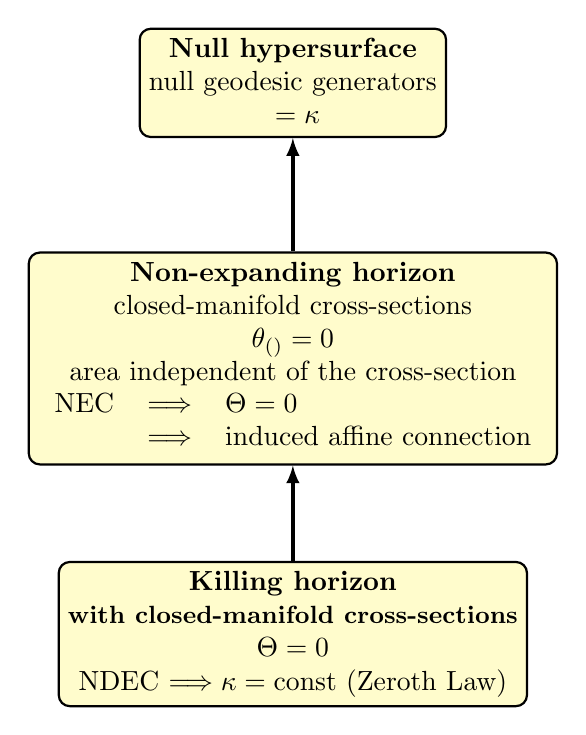
\begin{tikzpicture}
%\tikzstyle{boxst}=[rectangle,draw]
\tikzstyle{boxst}=[draw, thick, align=center, fill=yellow!20, rounded corners]
\tikzstyle{inherits}=[->,very thick,>=latex]
\node[boxst] (N) at (0,7) {\textbf{Null hypersurface}\\
null geodesic generators\\
$\wnab_{\wl}\wl = \kappa\wl$};
\node[boxst] (H) at (0,3.5) {\textbf{Non-expanding horizon}\\
closed-manifold cross-sections\\
$\theta_{(\wl)}=0$\\
area independent of the cross-section\\
\begin{tabular}{lcl}
NEC &$\Longrightarrow$ & $\w{\Theta}=0$ \\
 & $\Longrightarrow$ & induced affine connection
\end{tabular}
};
\node[boxst] (K) at (0,0) {\textbf{Killing horizon}\\
\textbf{\small with closed-manifold cross-sections}\\
$\w{\Theta}=0$ \\
NDEC $\Longrightarrow \kappa=\mathrm{const}$ (Zeroth Law)};
\draw[inherits] (H)--(N);
\draw[inherits] (K)--(H);
\end{tikzpicture}

\end{center}
